%%
%% Beginning of file 'sample61.tex'
%%
%% Modified 2016 September
%%
%% This is a sample manuscript marked up using the
%% AASTeX v6.1 LaTeX 2e macros. 
%%
%% This file was created on Overleaf.com
%%
%% AASTeX is now based on Alexey Vikhlinin's emulateapj.cls 
%% (Copyright 2000-2015).  See the classfile for details.

%% AASTeX requires revtex4-1.cls (http://publish.aps.org/revtex4/) and
%% other external packages (latexsym, graphicx, amssymb, longtable, and epsf).
%% All of these external packages should already be present in the modern TeX 
%% distributions.  If not they can also be obtained at www.ctan.org.

%% The first piece of markup in an AASTeX v6.x document is the \documentclass
%% command. LaTeX will ignore any data that comes before this command. The 
%% documentclass can take an optional argument to modify the output style.
%% The command below calls the preprint style  which will produce a tightly 
%% typeset, one-column, single-spaced document.  It is the default and thus
%% does not need to be explicitly stated.
%%
%%
%% using aastex version 6.1
\documentclass[twocolumn]{aastex61}

%% The default is a single spaced, 10 point font, single spaced article.
%% There are 5 other style options available via an optional argument. They
%% can be envoked like this:
%%
%% \documentclass[argument]{aastex61}
%% 
%% where the arguement options are:
%%
%%  twocolumn   : two text columns, 10 point font, single spaced article.
%%                This is the most compact and represent the final published
%%                derived PDF copy of the accepted manuscript from the publisher
%%  manuscript  : one text column, 12 point font, double spaced article.
%%  preprint    : one text column, 12 point font, single spaced article.  
%%  preprint2   : two text columns, 12 point font, single spaced article.
%%  modern      : a stylish, single text column, 12 point font, article with
%% 		  wider left and right margins. This uses the Daniel
%% 		  Foreman-Mackey and David Hogg design.
%%





%% Note that you can submit to the AAS Journals in any of these 6 styles.
%%
%% There are other optional arguments one can envoke to allow other stylistic
%% actions. The available options are:
%%
%%  astrosymb    : Loads Astrosymb font and define \astrocommands. 
%%  tighten      : Makes baselineskip slightly smaller, only works with 
%%                 the twocolumn substyle.
%%  times        : uses times font instead of the default
%%  linenumbers  : turn on lineno package.
%%  trackchanges : required to see the revision mark up and print its output
%%  longauthor   : Do not use the more compressed footnote style (default) for 
%%                 the author/collaboration/affiliations. Instead print all
%%                 affiliation information after each name. Creates a much
%%                 long author list but may be desirable for short author papers
%%
%% these can be used in any combination, e.g.
%%
%% \documentclass[twocolumn,linenumbers,trackchanges]{aastex61}

%% AASTeX v6.* now includes \hyperref support. While we have built in specific
%% defaults into the classfile you can manually override them with the
%% \hypersetup command. For example,
%%
%%\hypersetup{linkcolor=red,citecolor=green,filecolor=cyan,urlcolor=magenta}
%%
%% will change the color of the internal links to red, the links to the
%% bibliography to green, the file links to cyan, and the external links to
%% magenta. Additional information on \hyperref options can be found here:
%% https://www.tug.org/applications/hyperref/manual.html#x1-40003

%% If you want to create your own macros, you can do so
%% using \newcommand. Your macros should appear before
%% the \begin{document} command.
%%
\usepackage{url}
\usepackage{enumitem} 
%\newcommand{\red}[1]{\textcolor{red}{#1}}
\newcommand{\red}[1]{{#1}}

\newcommand{\hMsun}{{\ifmmode{h^{-1}{\rm
        {M_{\odot}}}}\else{$h^{-1}{\rm{M_{\odot}}}$~}\fi}} 
\newcommand{\hMpc}{{\ifmmode{h^{-1}{\rm Mpc}}\else{$h^{-1}$Mpc }\fi}}
\def\be{\begin{equation}}
\def\ee{\end{equation}}
\def\ba{\begin{eqnarray}}
\def\ea{\end{eqnarray}}

%% Reintroduced the \received and \accepted commands from AASTeX v5.2
\received{November 6, 2017}
\revised{November 27, 2017}
\accepted{\today}
%% Command to document which AAS Journal the manuscript was submitted to.
%% Adds "Submitted to " the arguement.
\submitjournal{ApJ}
%\submitjournal{ApJS}
%\submitjournal{AJ}

%% Mark up commands to limit the number of authors on the front page.
%% Note that in AASTeX v6.1 a \collaboration call (see below) counts as
%% an author in this case.
%
%\AuthorCollaborationLimit=3
%
%% Will only show Schwarz, Muench and "the AAS Journals Data Scientist 
%% collaboration" on the front page of this example manuscript.
%%



%% Note that all of the author will be shown in the published article.
%% This feature is meant to be used prior to acceptance to make the
%% front end of a long author article more manageable. Please do not use
%% this functionality for manuscripts with less than 20 authors. Conversely,
%% please do use this when the number of authors exceeds 40.
%%
%% Use \allauthors at the manuscript end to show the full author list.
%% This command should only be used with \AuthorCollaborationLimit is used.

%% The following command can be used to set the latex table counters.  It
%% is needed in this document because it uses a mix of latex tabular and
%% AASTeX deluxetables.  In general it should not be needed.
%\setcounter{table}{1}

%%%%%%%%%%%%%%%%%%%%%%%%%%%%%%%%%%%%%%%%%%%%%%%%%%%%%%%%%%%%%%%%%%%%%%%%%%%%%%%%
%%
%% The following section outlines numerous optional output that
%% can be displayed in the front matter or as running meta-data.
%%
%% If you wish, you may supply running head information, although
%% this information may be modified by the editorial offices.
\shorttitle{Cosmological parameter estimation from large-scale structure machine learning}
%%
%% You can add a light gray and diagonal water-mark to the first page 
%% with this command:
% \watermark{text}
%% where "text", e.g. DRAFT, is the text to appear.  If the text is 
%% long you can control the water-mark size with:
%  \setwatermarkfontsize{dimension}
%% where dimension is any recognized LaTeX dimension, e.g. pt, in, etc.
%%
%%%%%%%%%%%%%%%%%%%%%%%%%%%%%%%%%%%%%%%%%%%%%%%%%%%%%%%%%%%%%%%%%%%%%%%%%%%%%%%%

%% This is the end of the preamble.  Indicate the beginning of the
%% manuscript itself with \begin{document}.

\begin{document}

\title{Cosmological parameter estimation from large-scale structure machine learning}

%% LaTeX will automatically break titles if they run longer than
%% one line. However, you may use \\ to force a line break if
%% you desire. In v6.1 you can include a footnote in the title.

%% A significant change from earlier AASTEX versions is in the structure for 
%% calling author and affilations. The change was necessary to implement 
%% autoindexing of affilations which prior was a manual process that could 
%% easily be tedious in large author manuscripts.
%%
%% The \author command is the same as before except it now takes an optional
%% arguement which is the 16 digit ORCID. The syntax is:
%% \author[xxxx-xxxx-xxxx-xxxx]{Author Name}
%%
%% This will hyperlink the author name to the author's ORCID page. Note that
%% during compilation, LaTeX will do some limited checking of the format of
%% the ID to make sure it is valid.
%%
%% Use \affiliation for affiliation information. The old \affil is now aliased
%% to \affiliation. AASTeX v6.1 will automatically index these in the header.
%% When a duplicate is found its index will be the same as its previous entry.
%%
%% Note that \altaffilmark and \altaffiltext have been removed and thus 
%% can not be used to document secondary affiliations. If they are used latex
%% will issue a specific error message and quit. Please use multiple 
%% \affiliation calls for to document more than one affiliation.
%%
%% The new \altaffiliation can be used to indicate some secondary information
%% such as fellowships. This command produces a non-numeric footnote that is
%% set away from the numeric \affiliation footnotes.  NOTE that if an
%% \altaffiliation command is used it must come BEFORE the \affiliation call,
%% right after the \author command, in order to place the footnotes in
%% the proper location.
%%
%% Use \email to set provide email addresses. Each \email will appear on its
%% own line so you can put multiple email address in one \email call. A new
%% \correspondingauthor command is available in V6.1 to identify the
%% corresponding author of the manuscript. It is the author's responsibility
%% to make sure this name is also in the author list.
%%
%% While authors can be grouped inside the same \author and \affiliation
%% commands it is better to have a single author for each. This allows for
%% one to exploit all the new benefits and should make book-keeping easier.
%%
%% If done correctly the peer review system will be able to
%% automatically put the author and affiliation information from the manuscript
%% and save the corresponding author the trouble of entering it by hand.

\author{Shuyang Pan, Miaoxin Liu, Ziyong Wu, Haitao Miao, Xiaolin Luo, Xiao-Dong Li}
\affiliation{School of Physics and Astronomy, Sun Yat-Sen University, Guangzhou 510297, P.R.China}


\author{Cristiano G. Sabiu}
\affiliation{Department of Astronomy, Yonsei University, Seoul, Korea}

\author{Jaime Forero-Romero}
\affiliation{Departamento de F{\'i}sica, Universidad de los Andes, Cra. 1 No. 18A-10 Edificio Ip, CP 111711, Bogot{\'a}, Colombia}

\email{Corresponding Authors:  lixiaod25@mail.sysu.edu.cn}


%% Note that the \and command from previous versions of AASTeX is now
%% depreciated in this version as it is no longer necessary. AASTeX 
%% automatically takes care of all commas and "and"s between authors names.

%% AASTeX 6.1 has the new \collaboration and \nocollaboration commands to
%% provide the collaboration status of a group of authors. These commands 
%% can be used either before or after the list of corresponding authors. The
%% argument for \collaboration is the collaboration identifier. Authors are
%% encouraged to surround collaboration identifiers with ()s. The 
%% \nocollaboration command takes no argument and exists to indicate that
%% the nearby authors are not part of surrounding collaborations.

%% Mark off the abstract in the ``abstract'' environment. 
\begin{abstract}
%We expect this can be achieved (or falsified) in near future aided by much more advanced LSS experiments.
%With less datasets than what included in \citep{Zhao:2017cud}, our constraint is weaker than their result at higher reshift ($z\gtrsim0.7$). In future works, it's interesting to include more datasets and re-perform this analysis.
\end{abstract}

%% Keywords should appear after the \end{abstract} command. 
%% See the online documentation for the full list of available subject
%% keywords and the rules for their use.
\keywords{large-scale structure of Universe --- dark energy --- cosmological parameters}

%% From the front matter, we move on to the body of the paper.
%% Sections are demarcated by \section and \subsection, respectively.
%% Observe the use of the LaTeX \label
%% command after the \subsection to give a symbolic KEY to the
%% subsection for cross-referencing in a \ref command.
%% You can use LaTeX's \ref and \label commands to keep track of
%% cross-references to sections, equations, tables, and figures.
%% That way, if you change the order of any elements, LaTeX will
%% automatically renumber them.

%% We recommend that authors also use the natbib \citep
%% and \citet commands to identify citations.  The citations are
%% tied to the reference list via symbolic KEYs. The KEY corresponds
%% to the KEY in the \bibitem in the reference list below. 


\section{Introduction}

Machine learning is useful ...

LSS is non-linear... 
To build the connection between the LSS and the underlyig cosmological parameters, machine learning should be useful...

Pioneering works have been done in \citep{Ravanbakhsh2017}. ...

We tested ...

%--------------------------------------------------------------------------------------------------------------
\section{Data}

Training sample:

$0.16 \leq \Omega_m \leq 0.46$, step size 0.01, 31 numbers;

$2.0 \leq 10^9 A_s \leq 2.3$, step size 0.02, 15 numbers;


For reference, Planck 2015 (TT,TE,EE+lowP+lensing) gives 
$\Omega_m = 0.3121 \pm 0.0087$, 
$10^9 A_s = 2.13 \pm 0.053$,
$\sigma_8 = 0.8150 \pm 0.0087$


In total 31*15 = 465 cosmologies


Each cosmology: one COLA simulation, $128^3$ particles, $256^3$ box, COLA simulation, 40 timesteps


Redshift $z=0$ sample used in machine learning.

Test sample:

sing-cosmology test: 500 BigMD cosmologies $(\Omega_m, \sigma_8)=(0.3072,0.8228)$.
multi-cosmology test: all settings the same as training, except that using different initial condition 





\begin{figure*}
   \centering{
   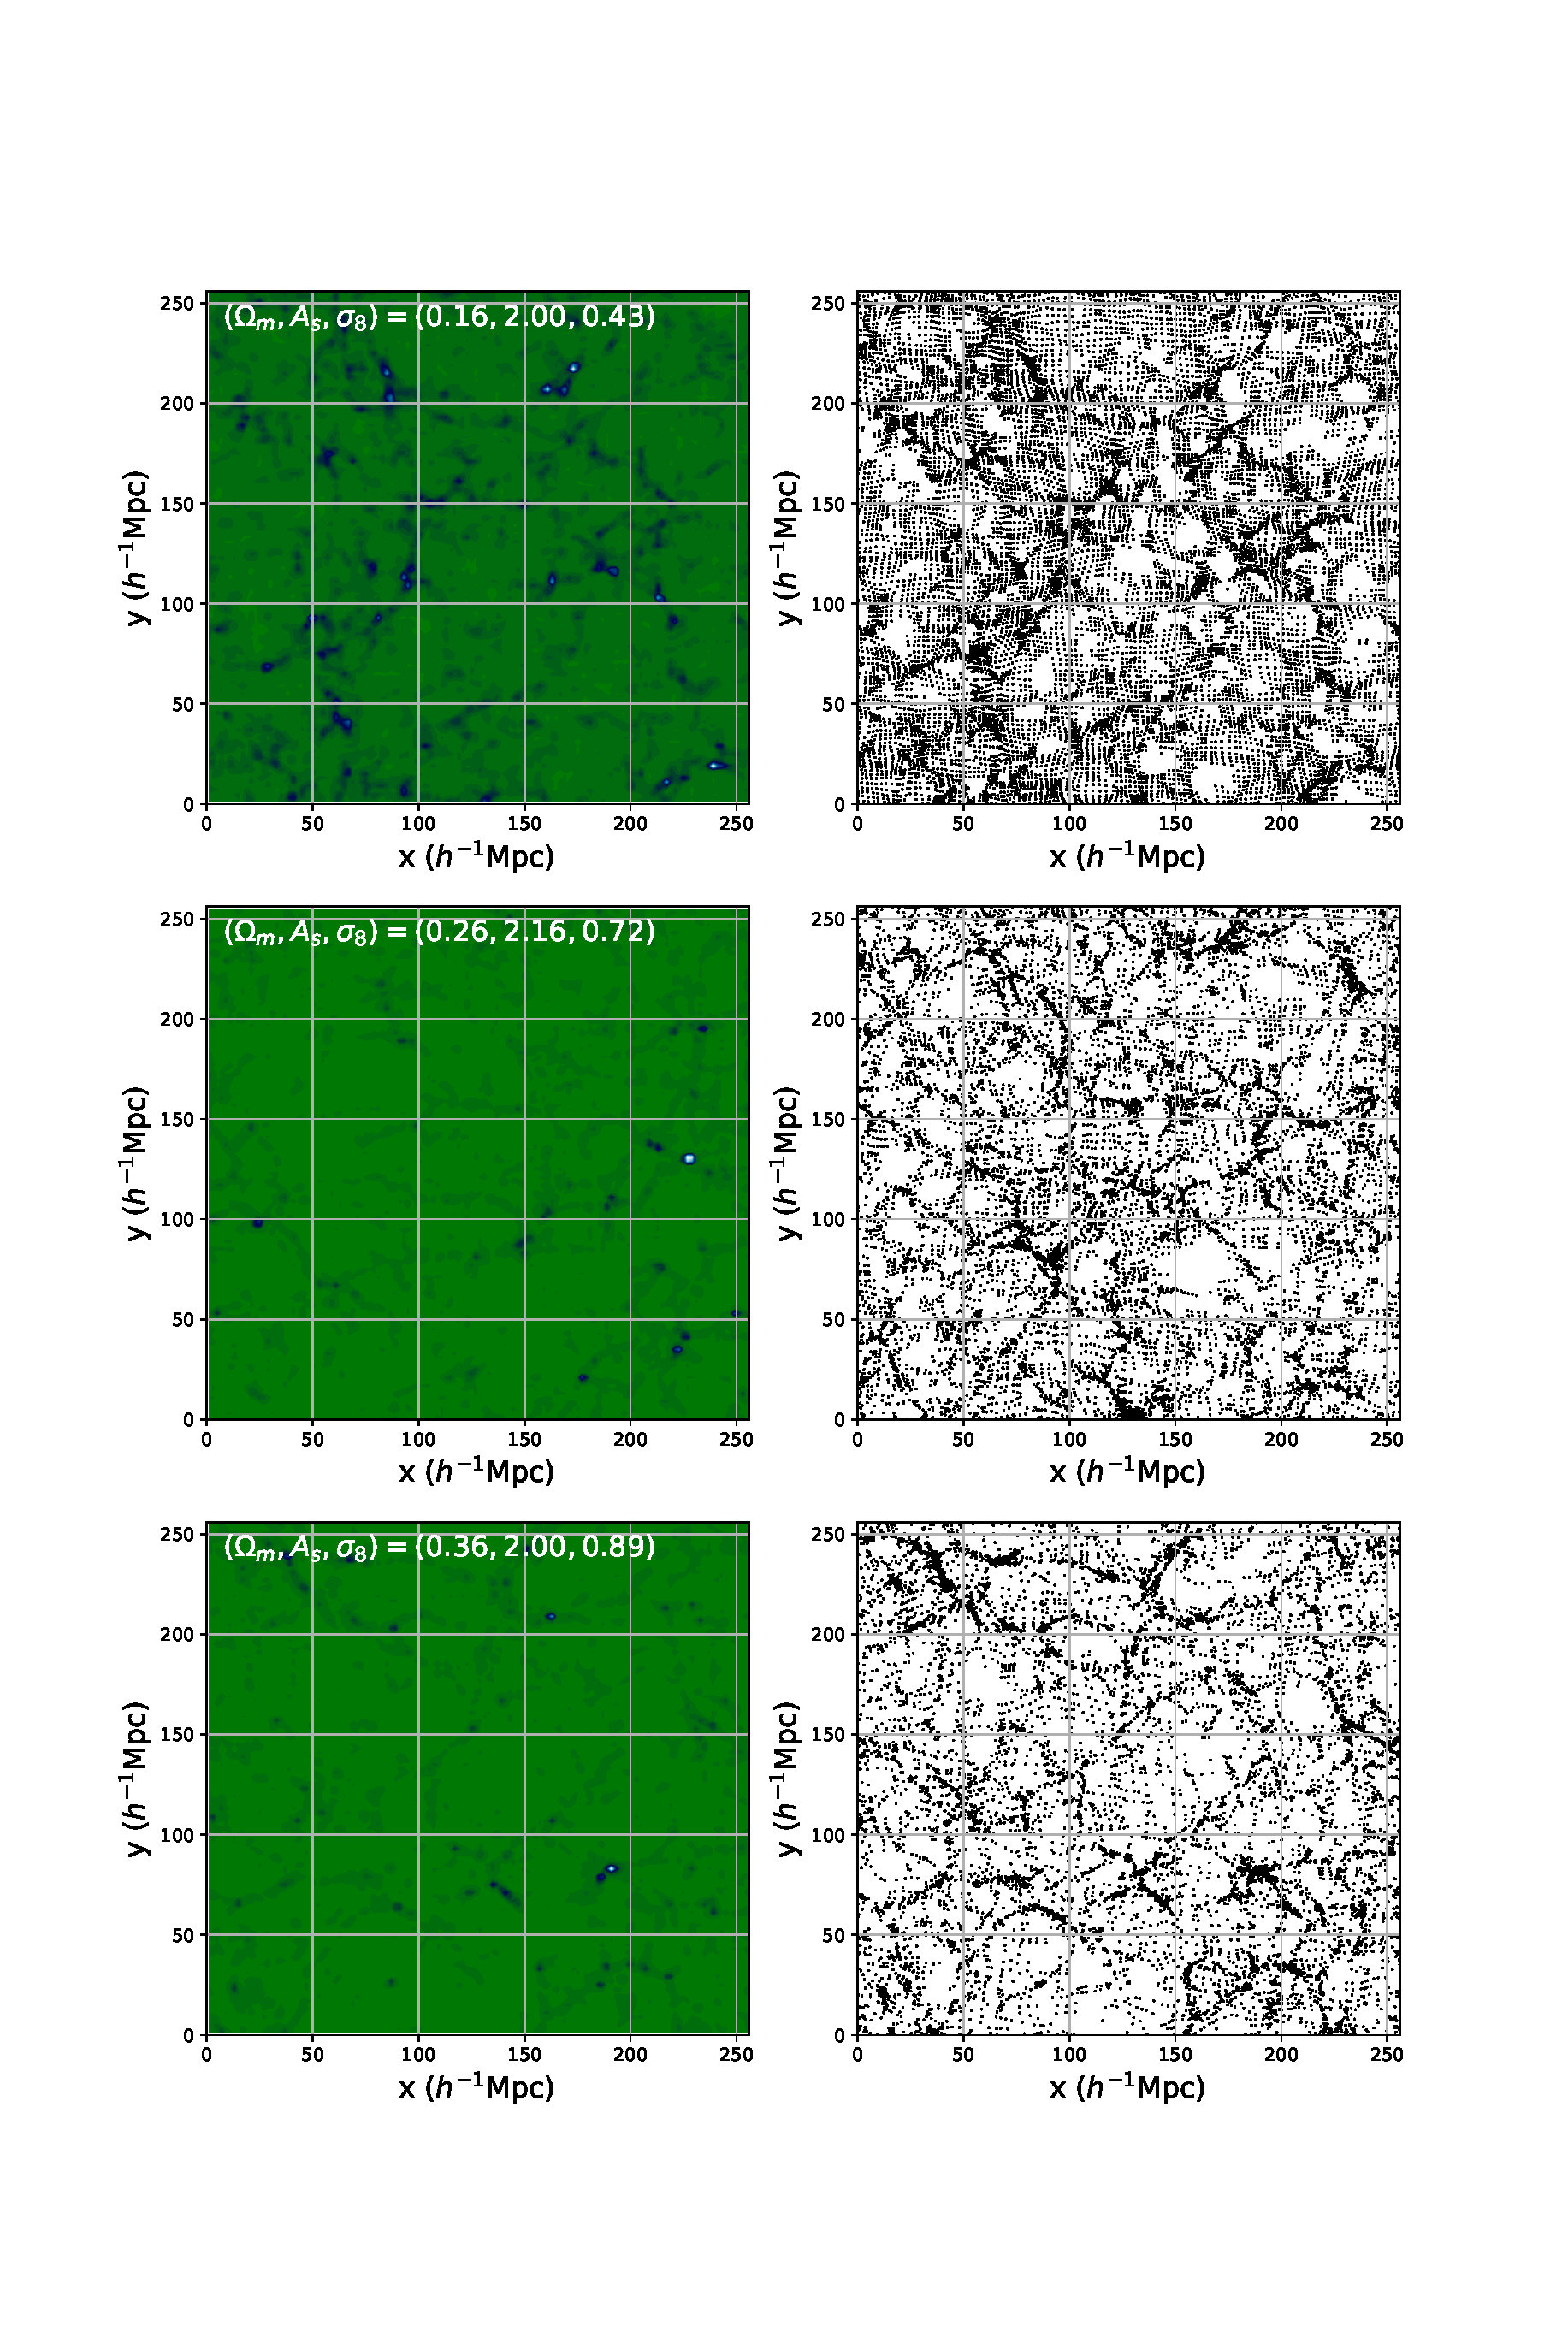
\includegraphics[width=12cm]{field.eps}
   }
   \caption{\label{fig_field}
   The density field (left) and particle distribution (right) of 
    three cosmologies 
    $(\Omega_m, A_s, \sigma_8)=(0.16,2,0.43),\ (0.26, 2.16, 0.72), (0.36, 2.0, 0.89)$,
    selected within the training sample.
   Thin slices with $0 h^{-1} {\rm Mpc}<z<2 h^{-1} {\rm Mpc}$ are plotted.
   The clustering strengh increases when increasing $\Omega_m$ or $A_s$, making the structures more compact.
   We train the neuron network to build up the connection between the density field and underlying cosmological parameters.
   }
\end{figure*}

\begin{figure*}
   \centering{
    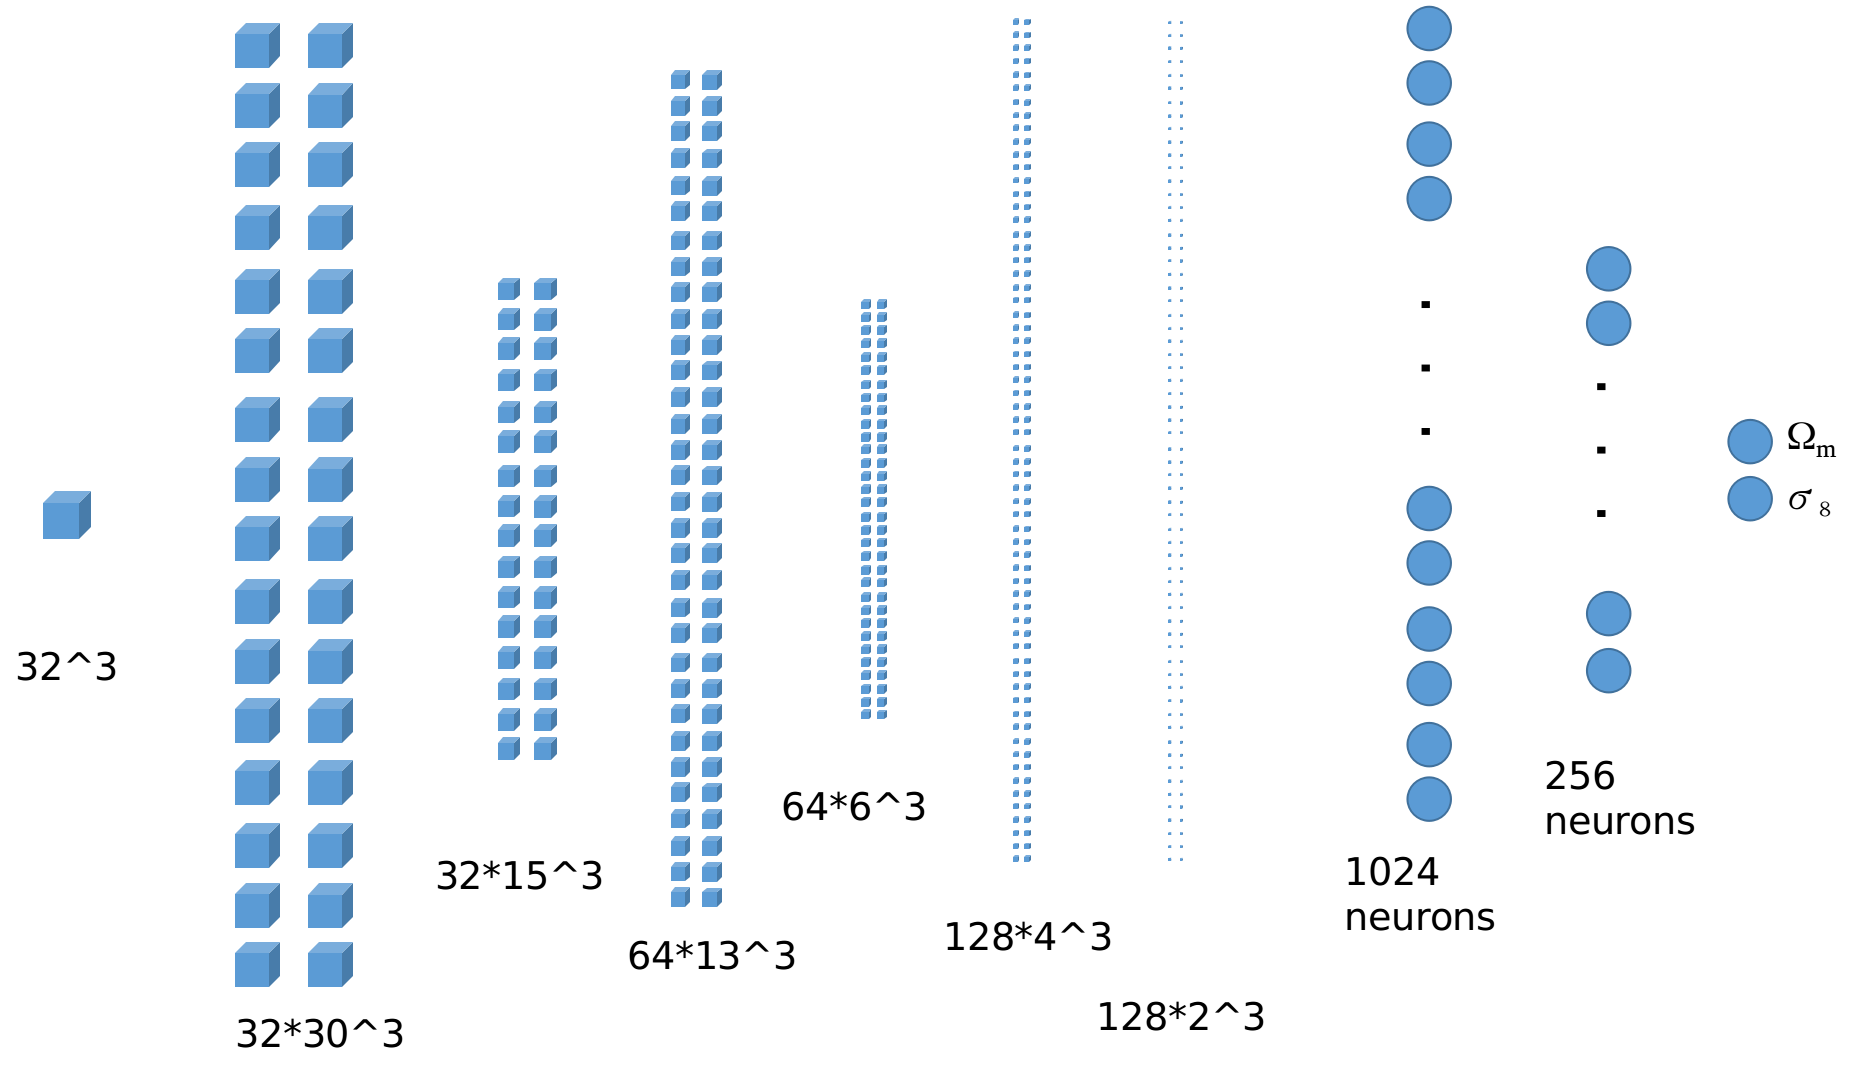
\includegraphics[width=12cm]{Picture1.png}
   }
   \caption{\label{fig_field}
   Architecture of our CNN (default settings).
   We split the $128^3$ voxels box into 64 sets of $32^3$ voxels sub-boxes, and then feed them to the CNN.
   After three convolution+pooling -- 
   with 32, 64, 128 filters in each convolution, respectively,
   we got $128\times 2^3$ voxels as the extracted features of the initial field.
   These voxels are then connected with three dense layers with 1028, 24 and 2 neurons,
   to predict $\Omega_m$ and $\sigma_8$.
   }
\end{figure*}

\begin{figure*}
   \centering
    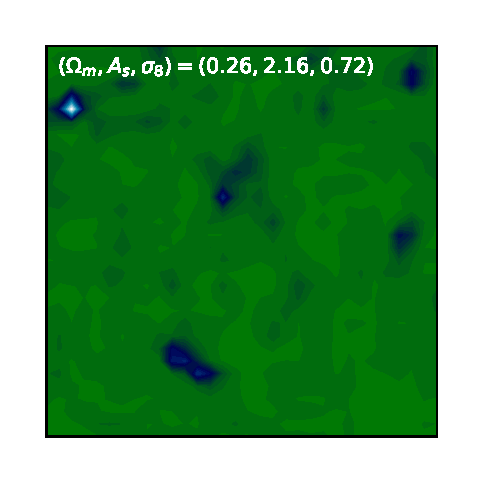
\includegraphics[height=4.5cm]{layeroutput_10.eps}
    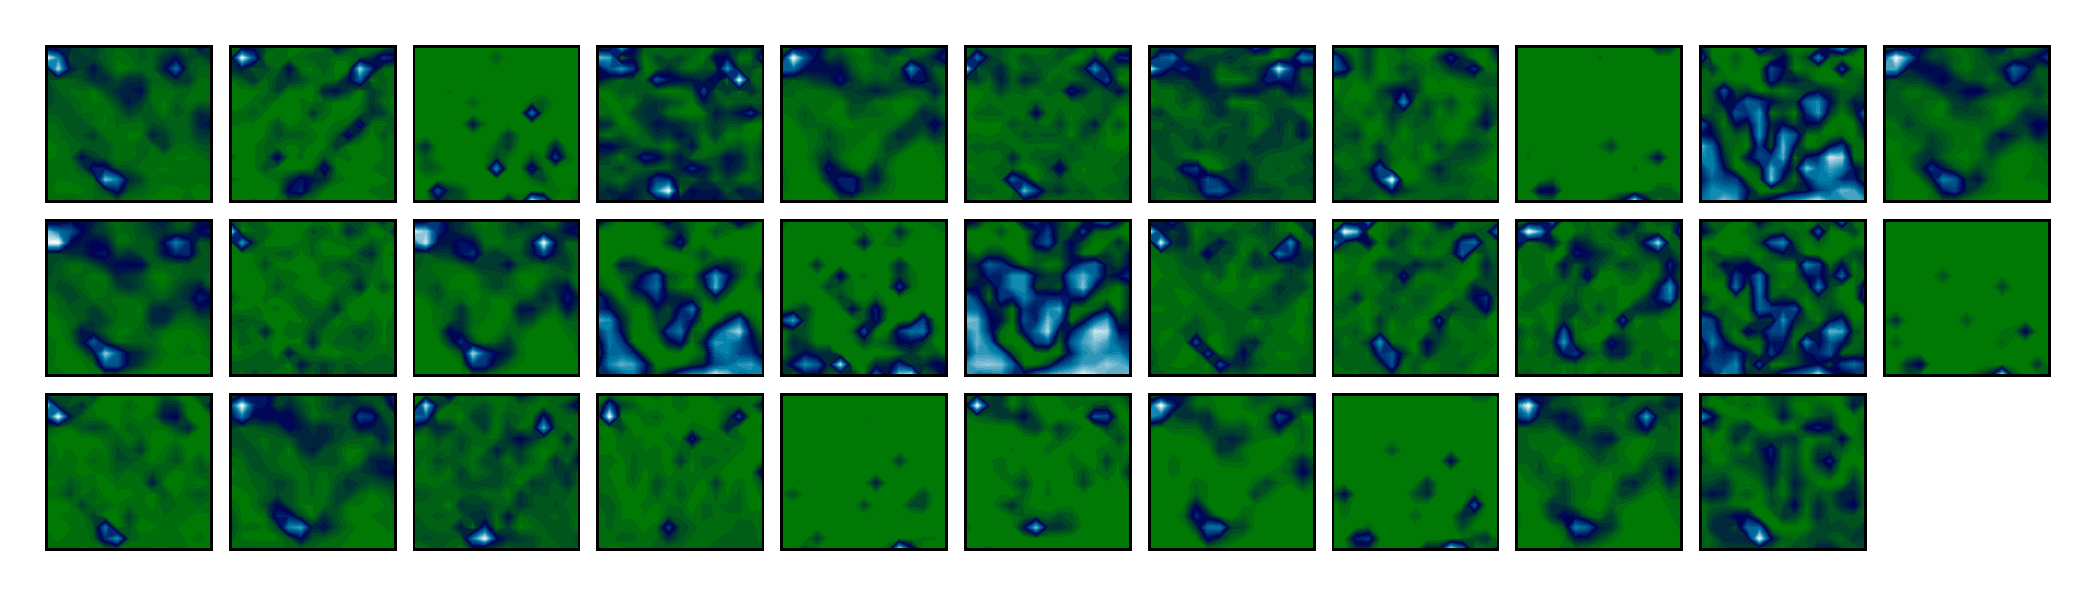
\includegraphics[height=4cm]{layeroutput_11.eps}
    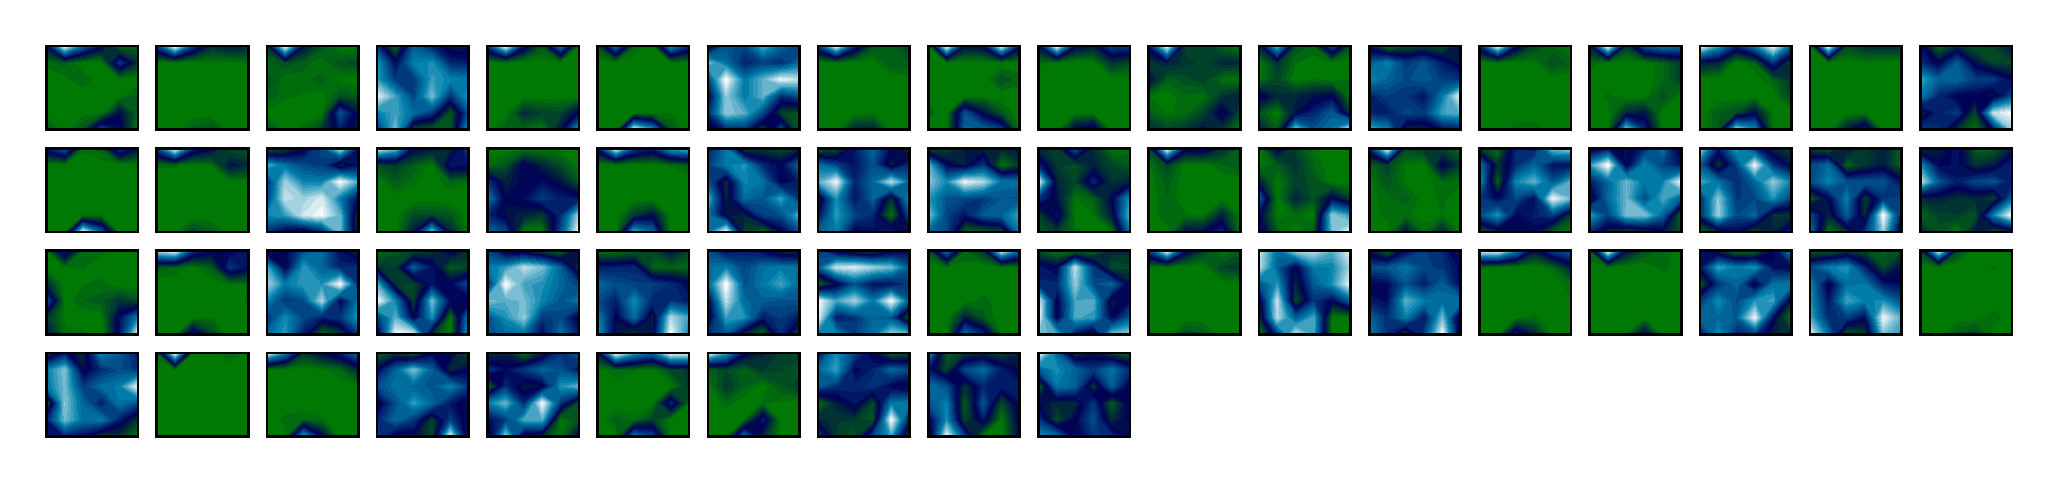
\includegraphics[height=3cm]{layeroutput_12.eps}
    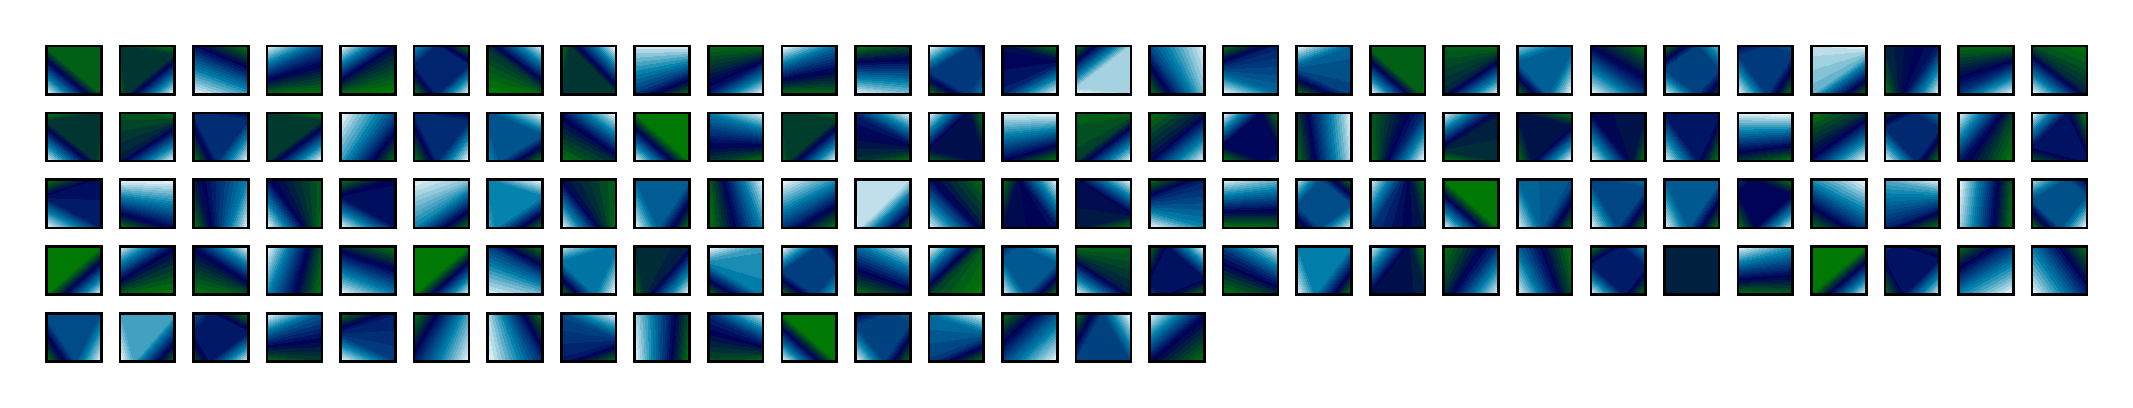
\includegraphics[height=2.5cm]{layeroutput_13.eps}
   \caption{\label{fig_layers1}
   Feature extraction in the CNN, taking the cosmology $(\Omega_m, A_s, \sigma_8)=(0.26, 2.16, 0.72)$ as the example. 
   The CNN was feeded with a $32^3$-box, whose $z<2 h^{-1} \rm Mpc$ slice is plotted in the uppermost panel.
   It was firstly convolved with 32 $3^3$-filters,
   and then pooled to generate 32 $15^3$-boxes.
   They capturing different types of features in the original box.
   Then, the 32 boxes are further convolved with 64 $3^3$-filters,
   which are also pooled to generate 64 $6^3$-boxes, 
   containing more compressed features.
   Finally, the last convolution+pooling outputs 128 $2^3$-boxes, 
   containing the most compressed information.
   These information are passed to the dense layers to produce 
   values of $\Omega_m$ and $\sigma_8$.
   The number of free parameters in the three convolutions are
   896, 55,360, 221,312, respectively.
   These free parameters are tuned in the training process 
    so that the convolutions can extract the features most sensitive to the 
    $\Omega_m$ and $\sigma_8$ values.
   }
\end{figure*}

\begin{figure*}
   \centering
    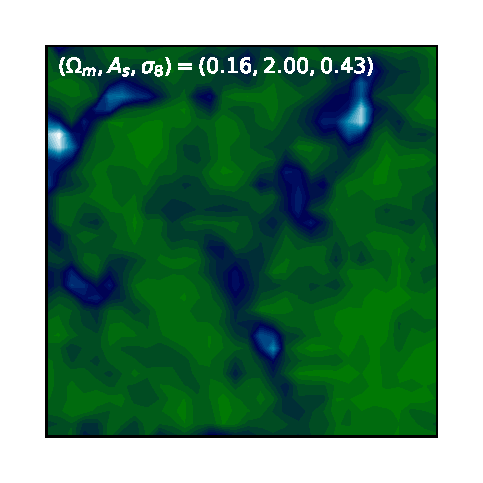
\includegraphics[height=4.5cm]{layeroutput_00.eps}
    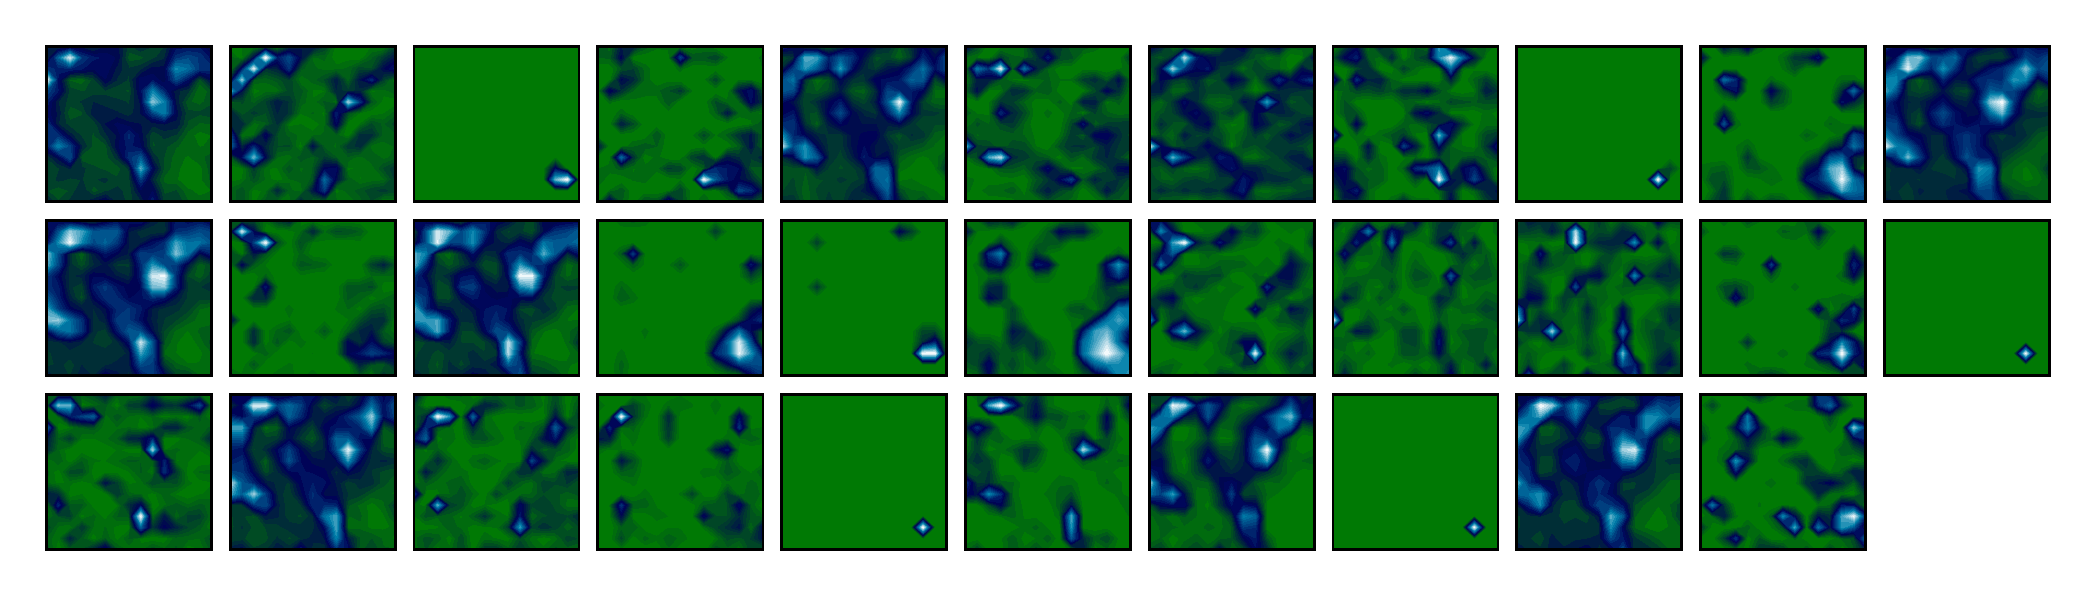
\includegraphics[height=4cm]{layeroutput_01.eps}
    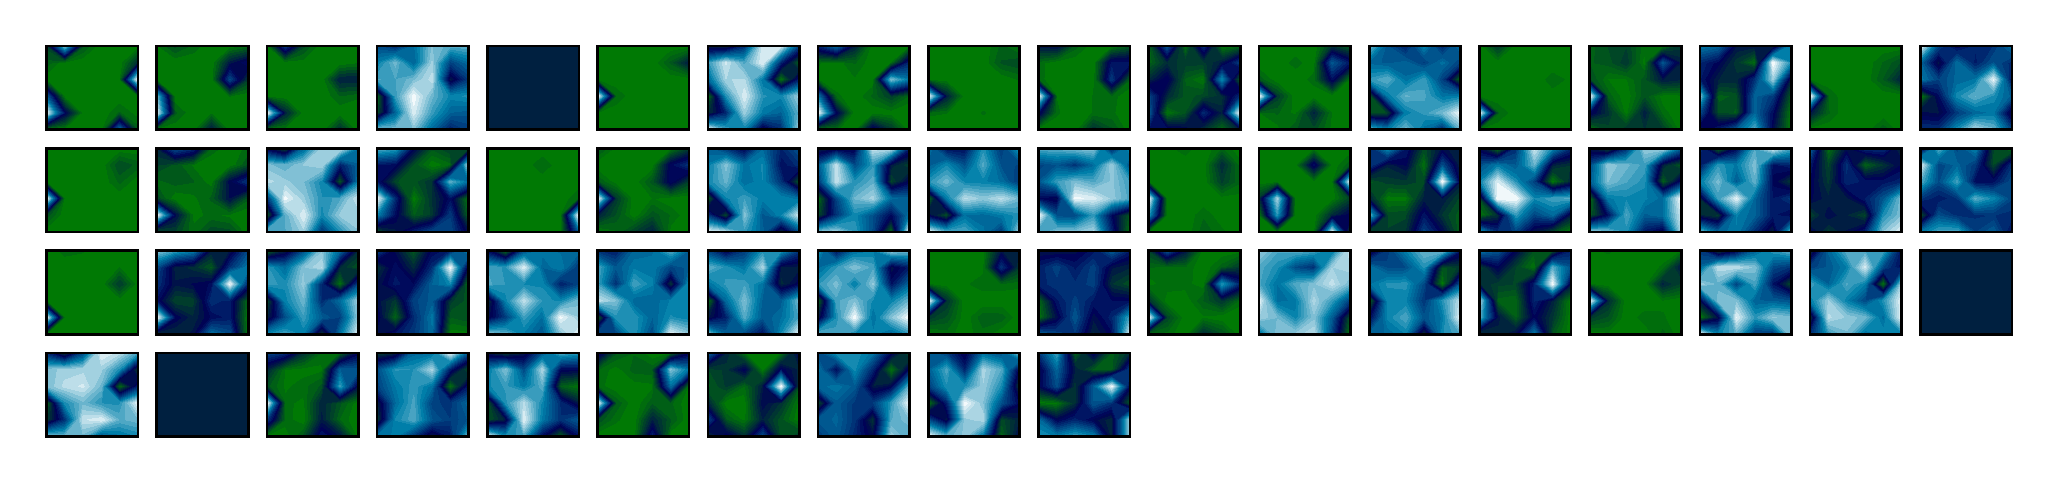
\includegraphics[height=3cm]{layeroutput_02.eps}
    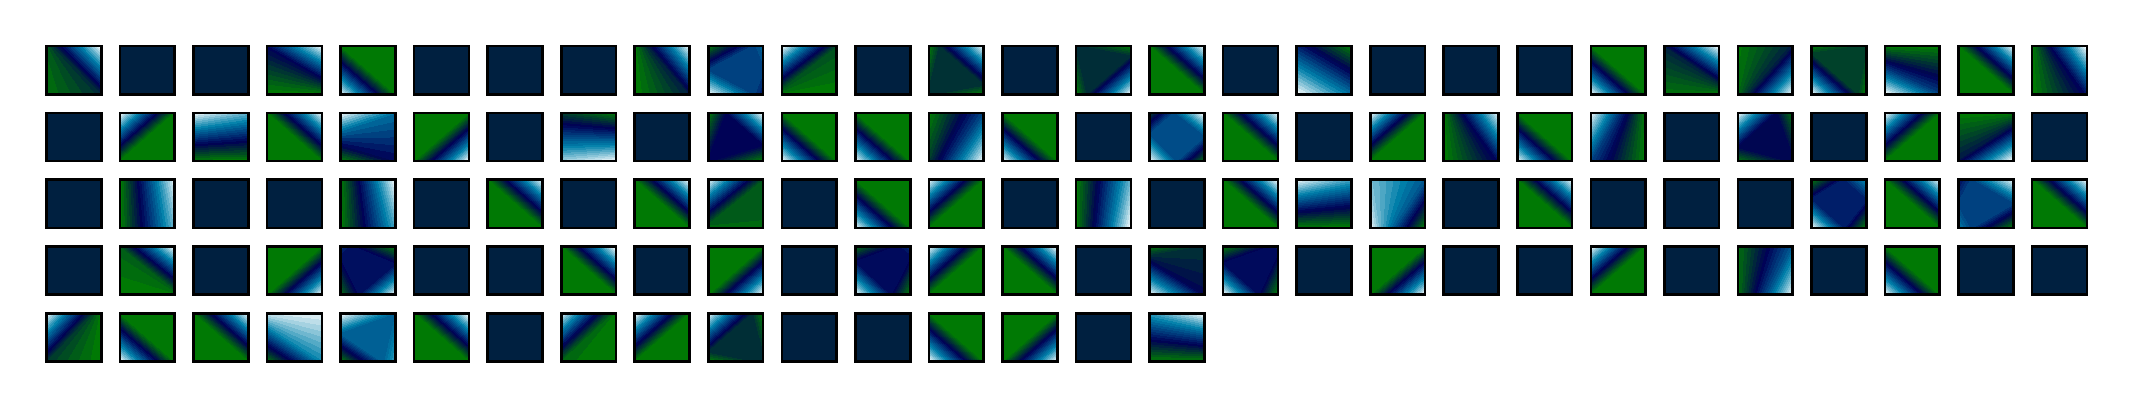
\includegraphics[height=2.5cm]{layeroutput_03.eps}
   \caption{\label{fig_layers2}
   The same as Figure \ref{fig_layers1}, except that the feature extraction was acted on the cosmology $(\Omega_m, A_s, \sigma_8)=(0.26, 2.00, 0.43)$. 
   The features extracted by the convolutions are different from those in the cosmology $(\Omega_m, A_s, \sigma_8)=(0.26, 2.16, 0.72)$.
   In this way, the CNN was able to tell that the input cosmology is different from the previous one, 
   and outputs different $\Omega_m$ and $\sigma_8$ values for different cosmologies.
   }
\end{figure*}

\begin{figure*}
   \centering
    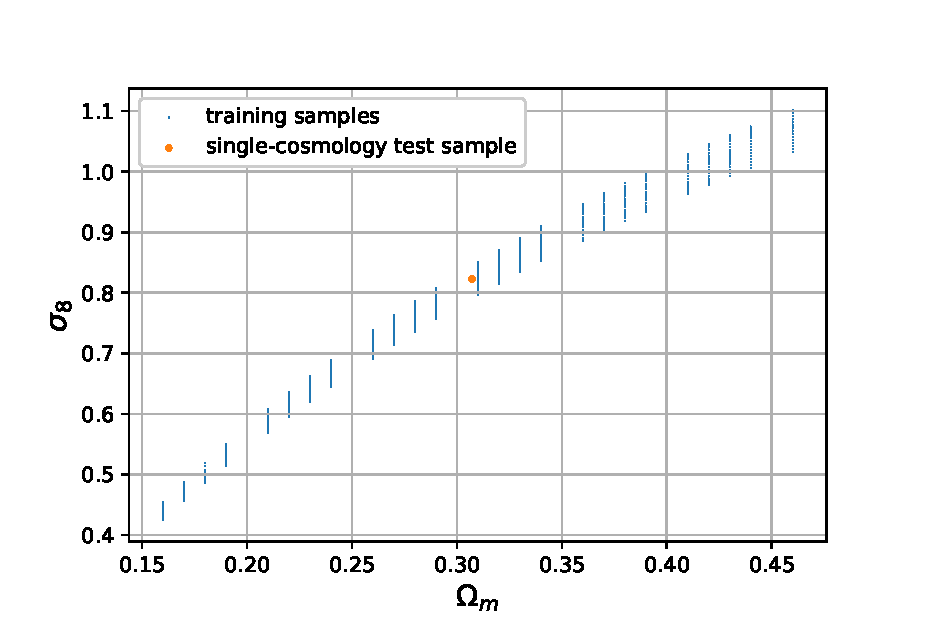
\includegraphics[height=8cm]{train_grid.eps}
   \caption{\label{fig_train_grid}
   Cosmological parameters of the 465 training samples (little blue dots) and single-cosmology test samples (big yellow dot).
   The multi-cosmology test samples have exactly the same parameters of the training samples, created using different initial conditions.
   }
\end{figure*}

\begin{figure*}
   \centering
    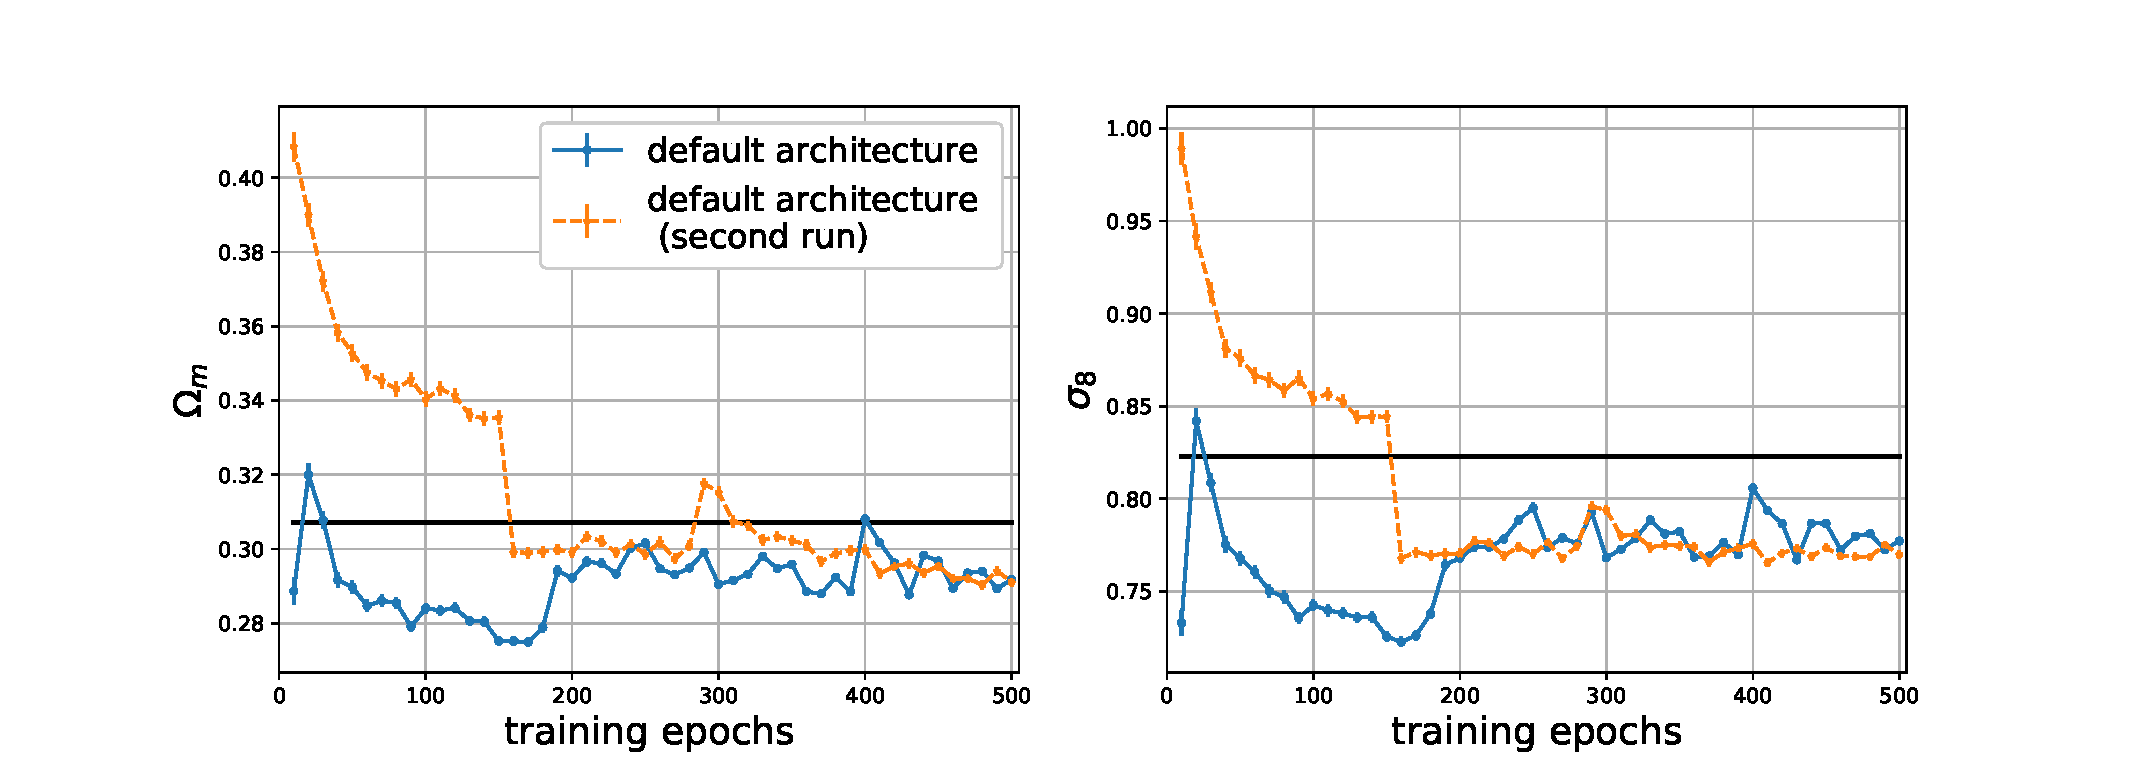
\includegraphics[height=6cm]{lc_default.eps}
   \caption{\label{lc_default}
   Learning curve using the default architecture (separately trained by two times), 
   tested on the single-cosmology samples.
   The underlying true cosmology parameters were marked by the thick black line.
   The outputs of CNN as a function of epochs are plotted in the blue solid and yellow dashed curves.
   The statistical errors (not quit visible after epochs > 200) are estimated using the variance of the outputs of the 500 realizations. 
   At the beginning of the training, 
   the behavior was bad and random;
   the performance then converge and become stable after 200 epochs training.
   The two separate training yield very similar results.
   Very roughly, the CNN has systematical errors of 0.02 and 0.05 in the estimation of $\Omega_m$ and $\sigma_8$
   }
\end{figure*}

\begin{figure*}
   \centering
    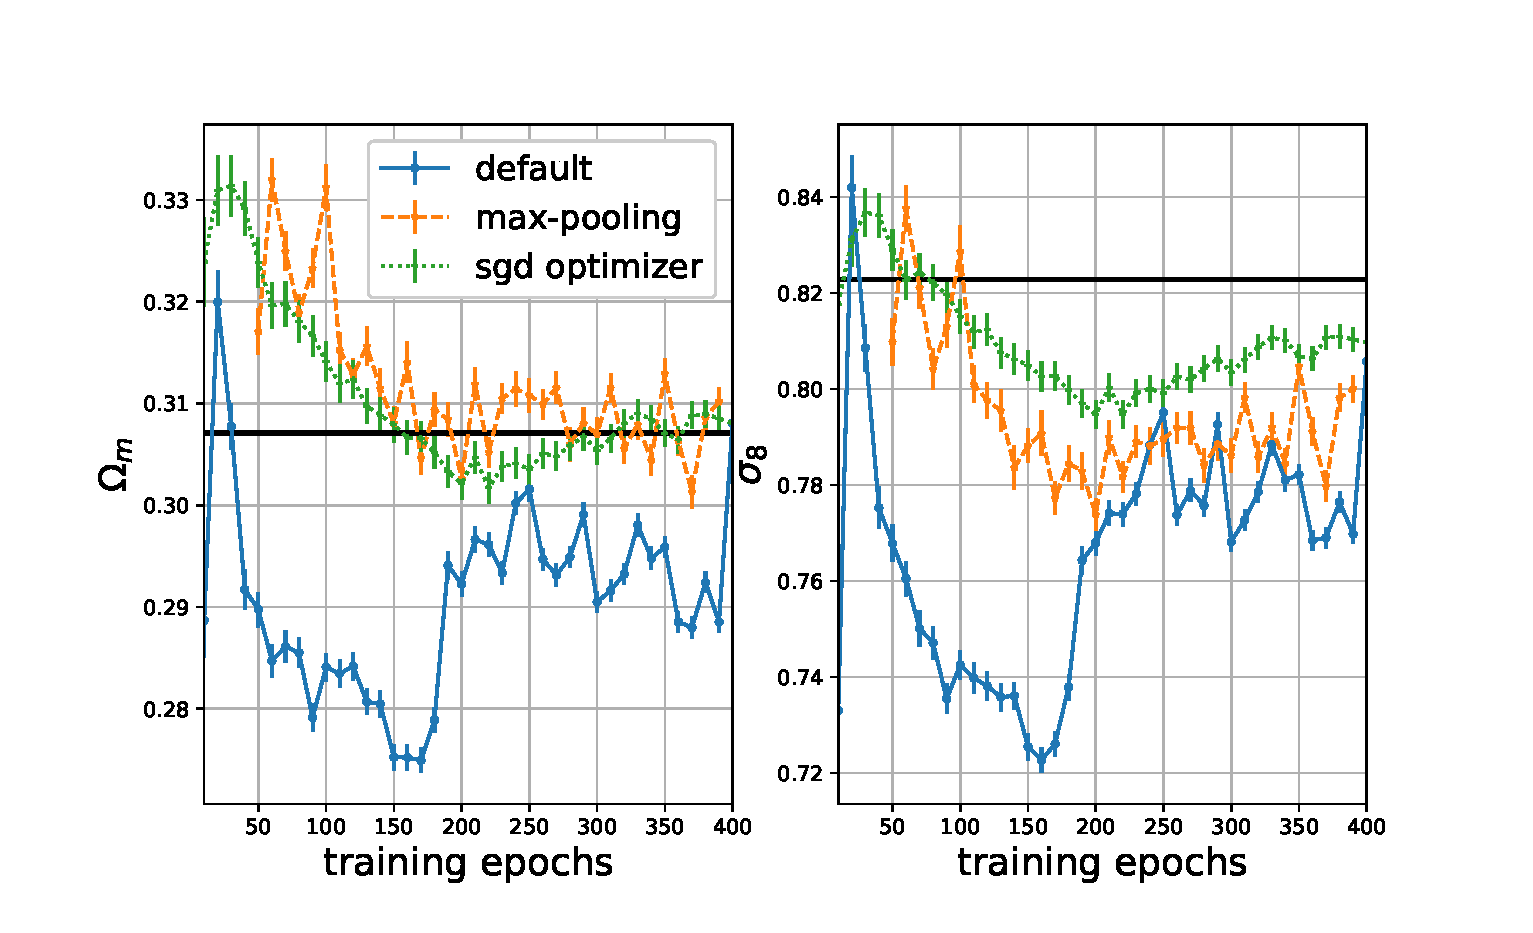
\includegraphics[height=5.3cm]{lc_sgdmaxpool.eps}
    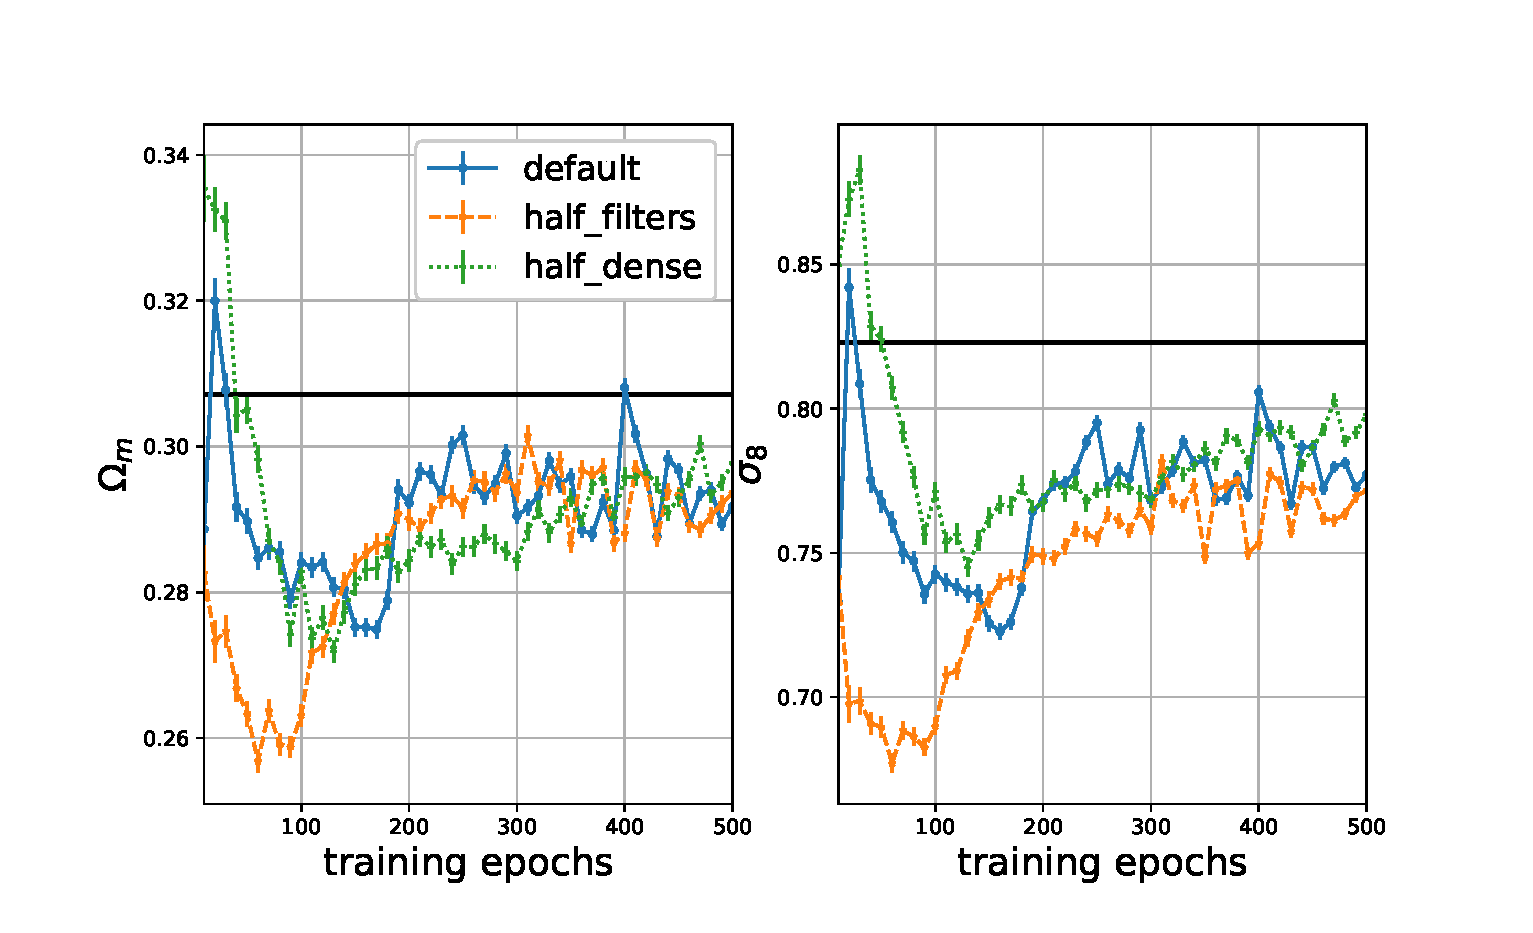
\includegraphics[height=5.3cm]{lc_half.eps}
   \caption{\label{lc_default}
   Learning curve using different settings of the CNN architecture and the optimization process.
   For comparison, the default settings are also plotted in the panels.
   {\it Left panel}: Using max-pooling rather than average-pooling in the pooling layer,
    the parameter estimation becomes better.
   This is different from the conclusion of \citep{Ravanbakhsh2017}, 
   where the authors got good estimations using average pooling, but failed to get reasonable parameter estimation using max-pooling.
   This should be due to the difference in the CNN architectures used in their and our paper
   \footnote{They use much less filters and more convolution layers.}.
   Also we find sgd (stochastic gradient descent) optimizer is helpful in improving the parameter estimation.
   Possibly, the default Adam optimizer enters local minimum and was trapped there.
   {\it Right panel}: Tests on the CNN architecture. 
   After decreasing the number of filters in the convolution layers (${\rm half\_filters}$),
   or the number of neurons in the dense layers (${\rm half\_dense}$), 
   the parameter estimation is, basically, as good as the default architecture.
   }
\end{figure*}

\begin{figure*}
   \centering
    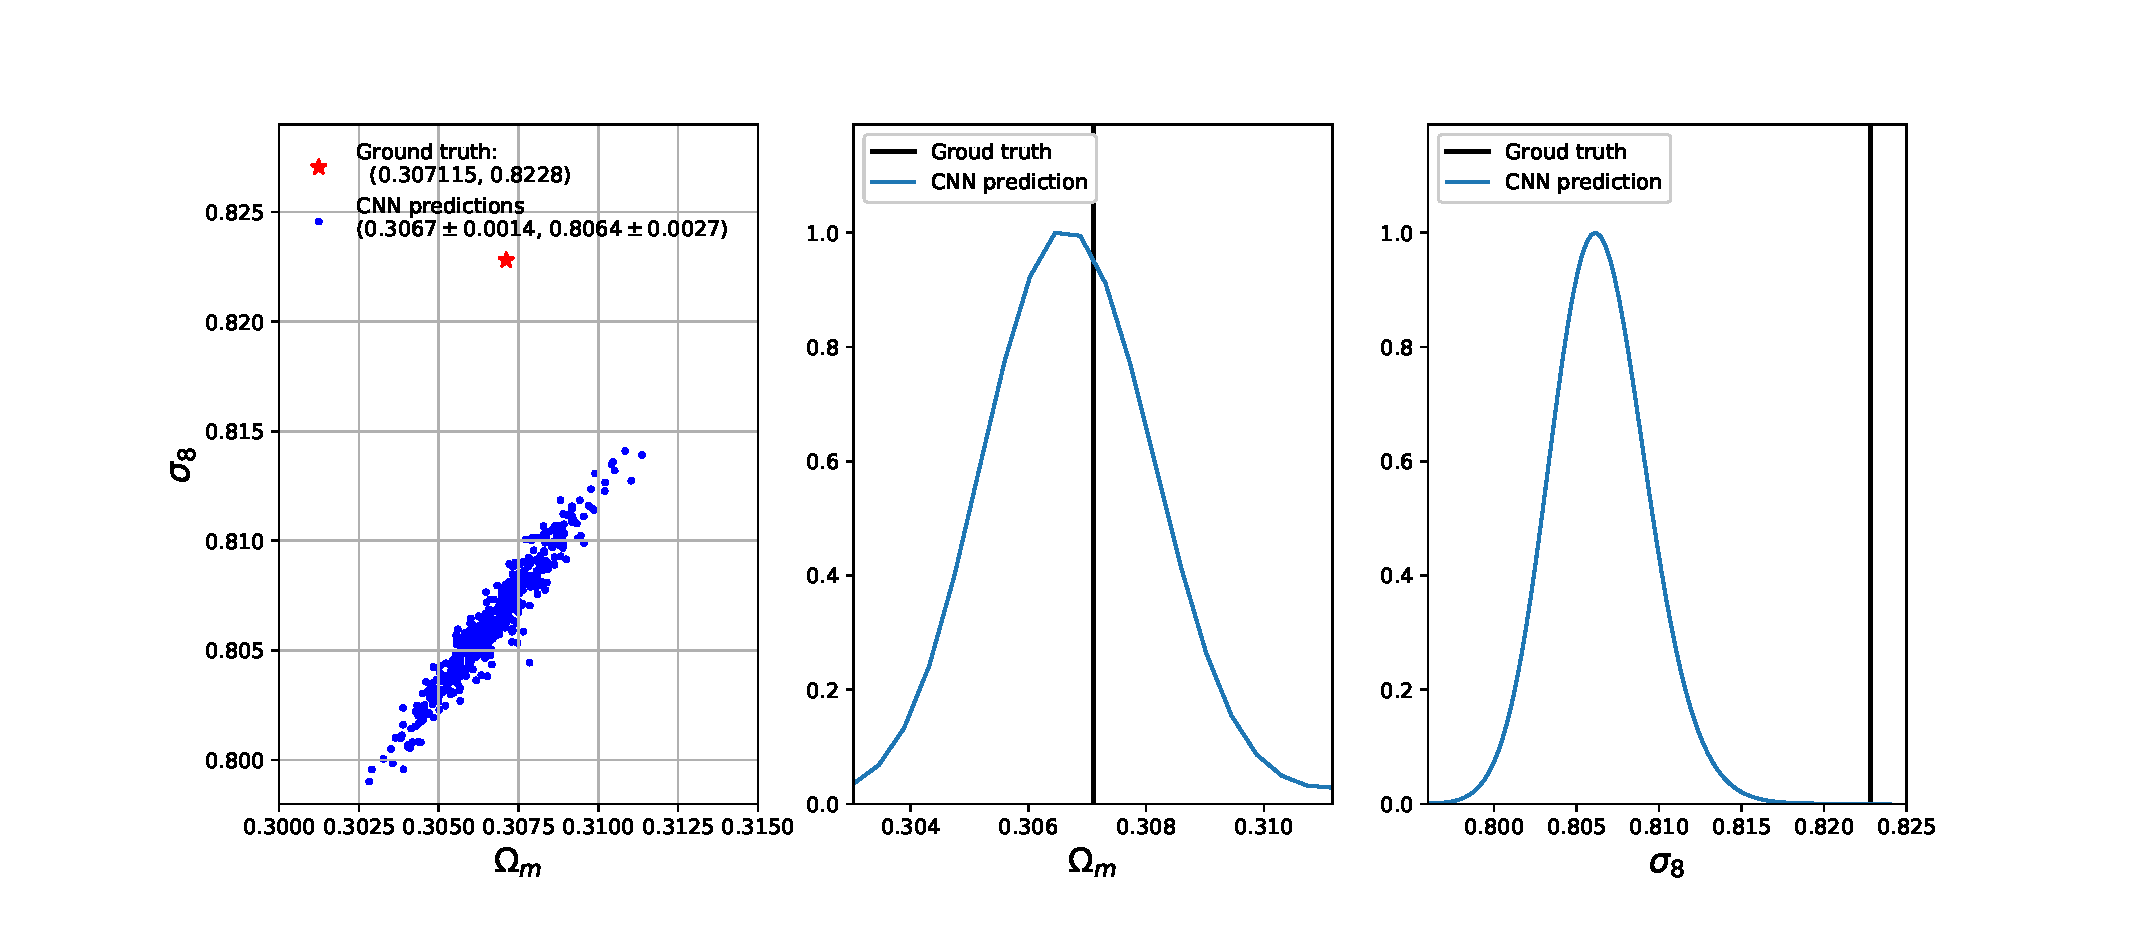
\includegraphics[width=16cm]{bigmd_rlt.eps}
   \caption{\label{single_cosmology}
   Test of a CNN architecture (sgd) on the single-cosmology samples.
   %There is a strong degeneracy between $\Omega_m$ and $\sigma_8$.
   {\it Left panel}: Ground truth (red star) and CNN predictions (blue dots) of $\Omega_m$ and $\sigma_8$, in the 2-d parameter space.
   The CNN well predicts the values of $\Omega_m$, but has a bias in estimating $\sigma_8$.
   {\it Middle and Right panels}: Likelihood distribution of $\Omega_m$, $\sigma_8$ from the CNN predictions.
   }
\end{figure*}

\begin{figure*}
   \centering
    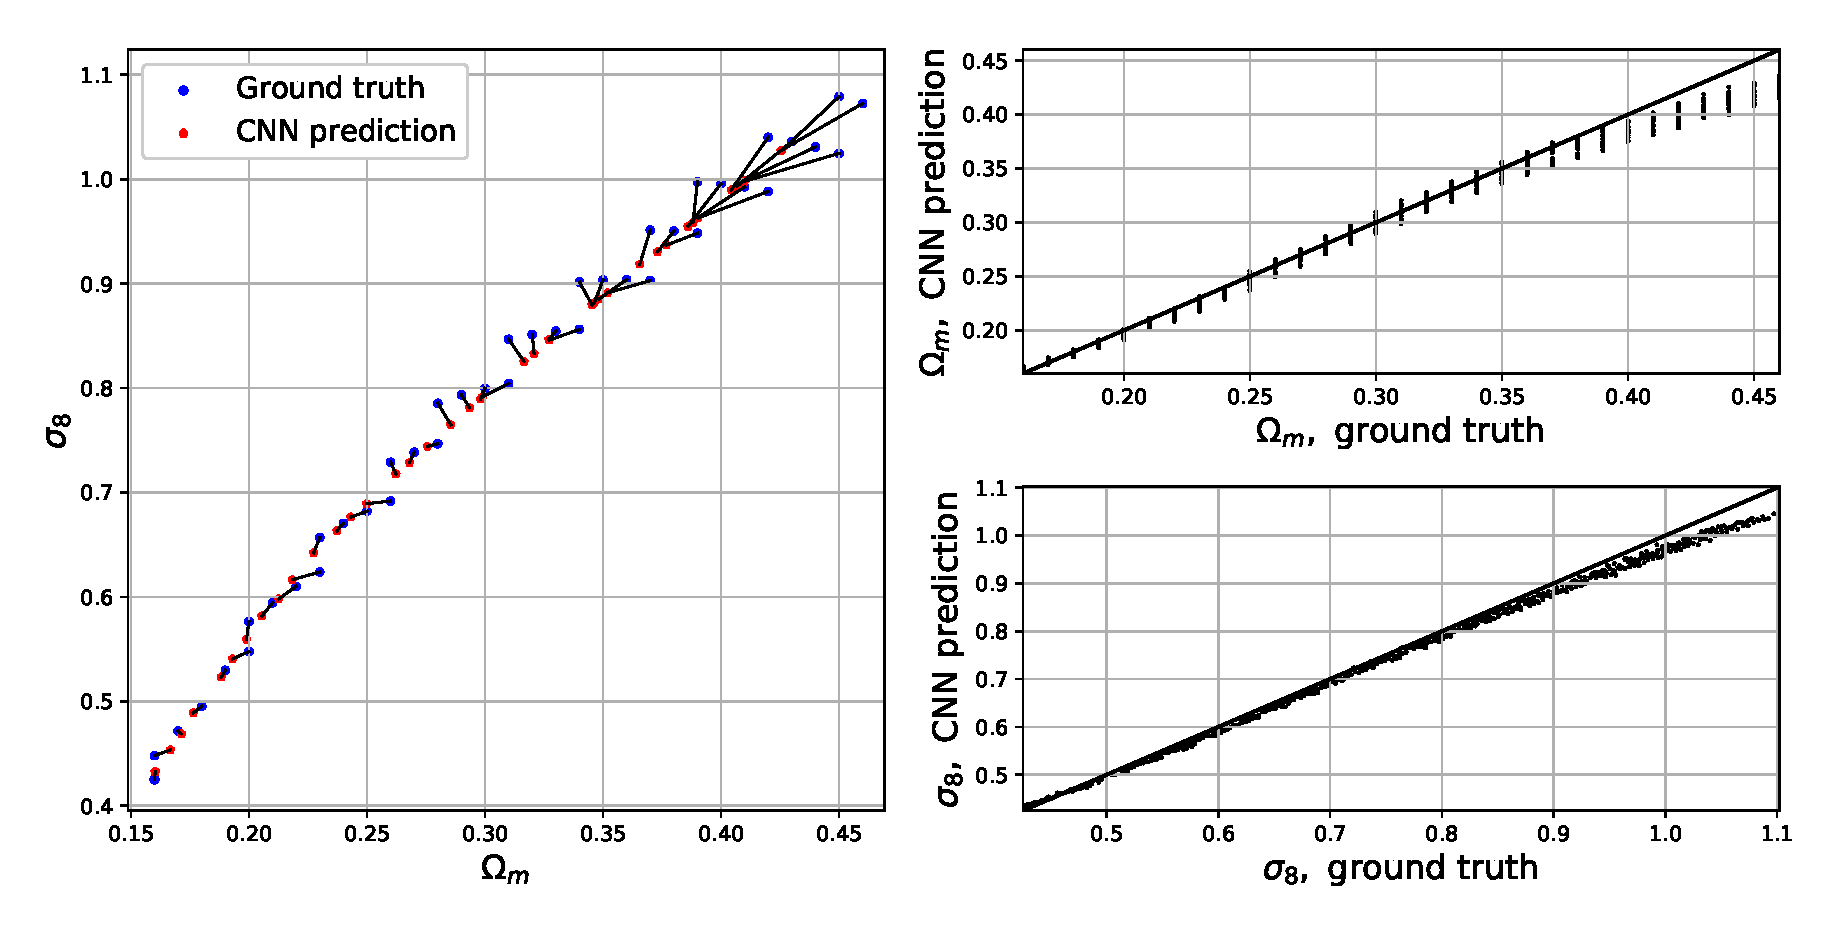
\includegraphics[width=16cm]{multi_cosmology.eps}
   \caption{\label{multi_cosmology}
   Test of a CNN architecture (sgd) on a multi-cosmology grid.
   There is a strong degeneracy between $\Omega_m$ and $\sigma_8$.
   {\it Left panel}: Ground truth and CNN predictions of $\Omega_m$ and $\sigma_8$, in the 2-d parameter space.
   The black lines show the difference between them.
   The error bar is larger at the upper-right corner of the parameter space.
   {\it Right panels}: Ground truth and CNN predictions for $\Omega_m$ and $\sigma_8$ panels, respectively.
   The CNN has slight under-estimation of the parameters at the large value tail.
   }
\end{figure*}

\begin{figure*}
   \centering
    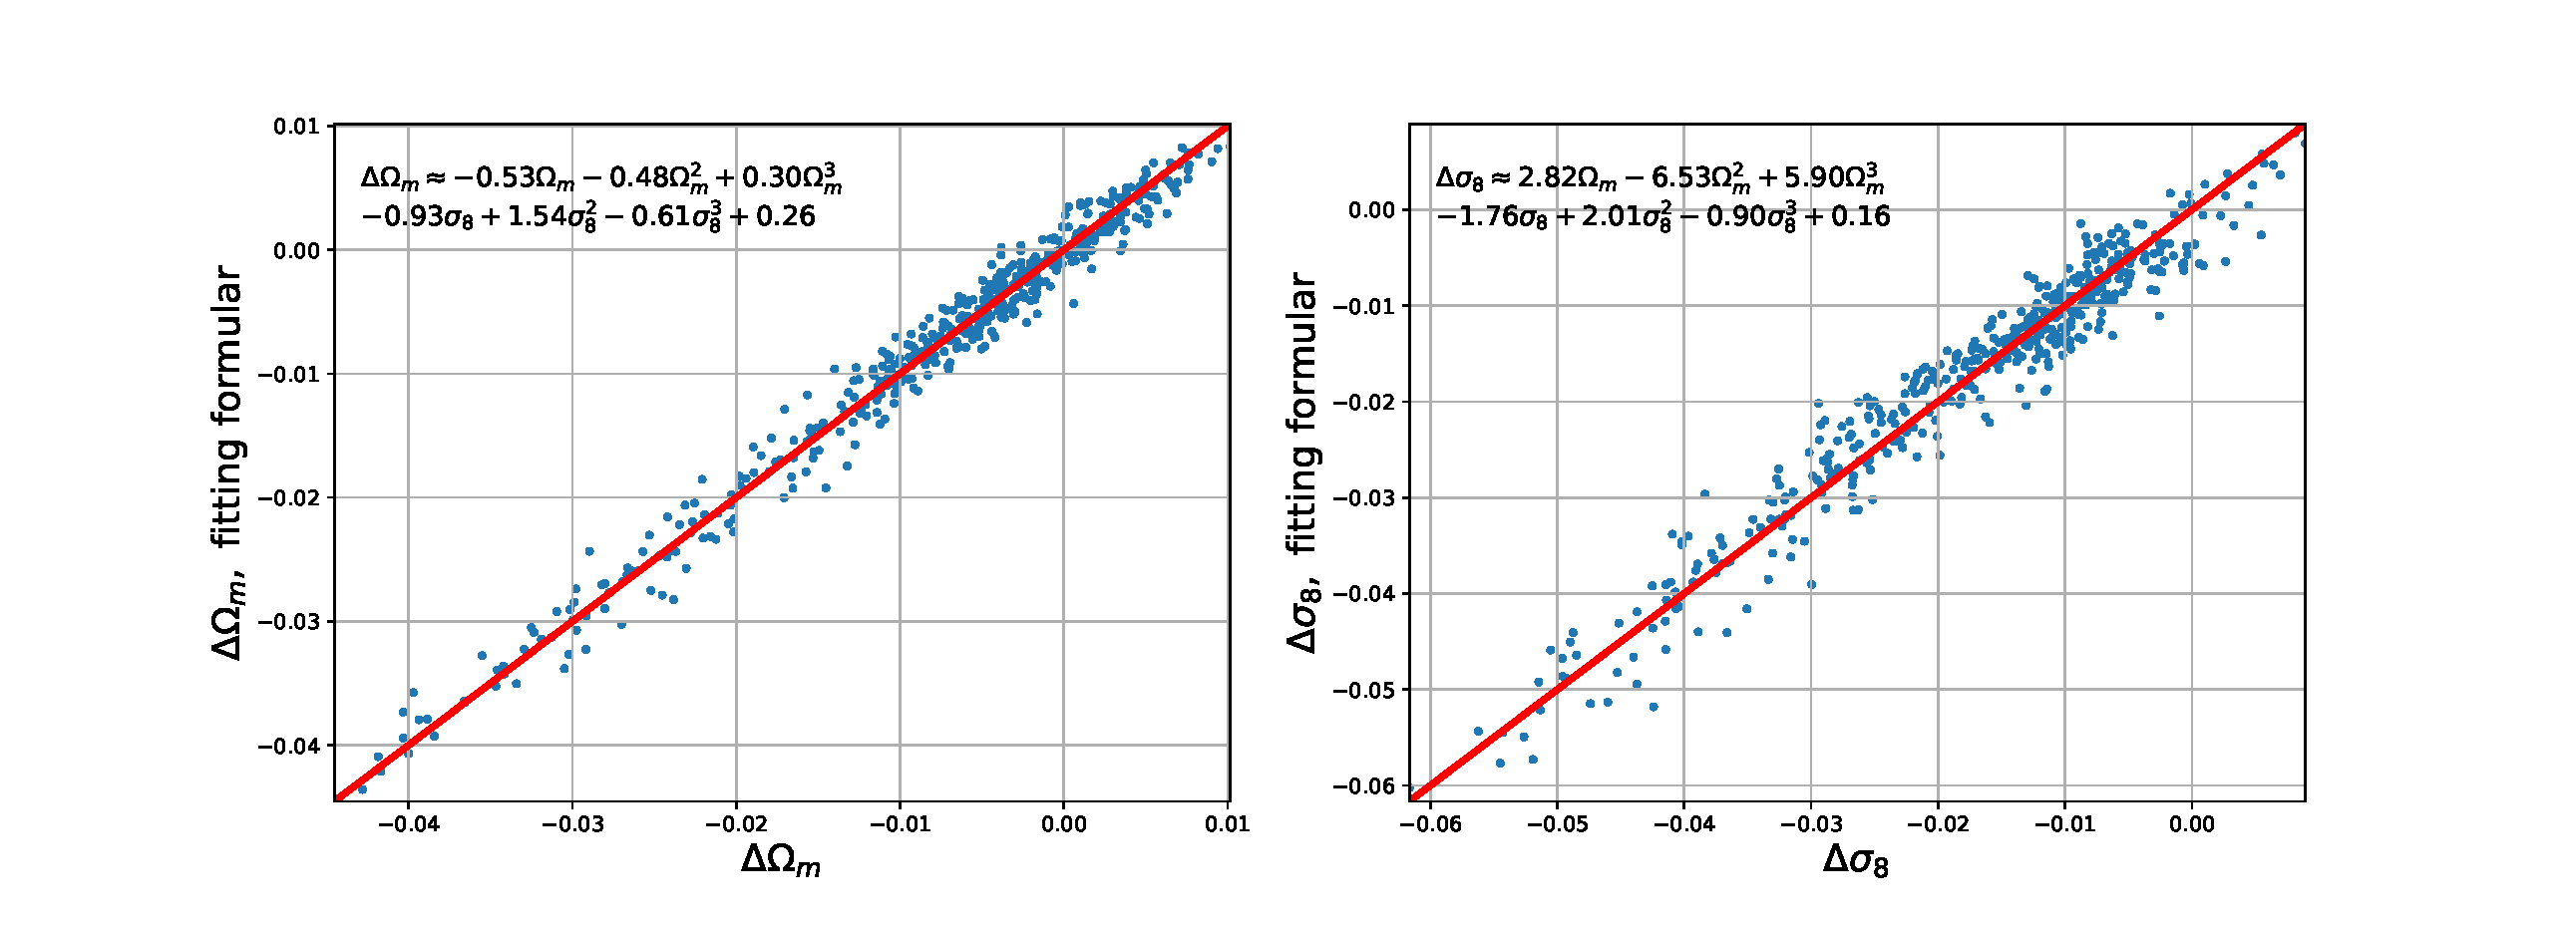
\includegraphics[width=16cm]{bias.eps}
   \caption{\label{bias}
   Distribution of the systematic bias in the CNN predicted $\Omega_m$ and $\sigma_8$ (denoted as $\Delta \Omega_m$ and $\Delta \sigma_8$).
   Very roughly, in the parameter space we studied, 
    there is $|\Delta \Omega_m| \lesssim 0.03$ and $|\Delta \sigma_8| \lesssim 0.05$,
    with mean value of $\bar|\Delta \Omega_m|=0.01$ and $\bar|\Delta \sigma_8|=0.018$.
   In practice one can calibrate the results by subtract the systematic bias in the CNN predictions (e.g., using the fitting formula shown in the panels), 
   making the final estimation unbiased.  
   }
\end{figure*}

\begin{figure*}
   \centering
    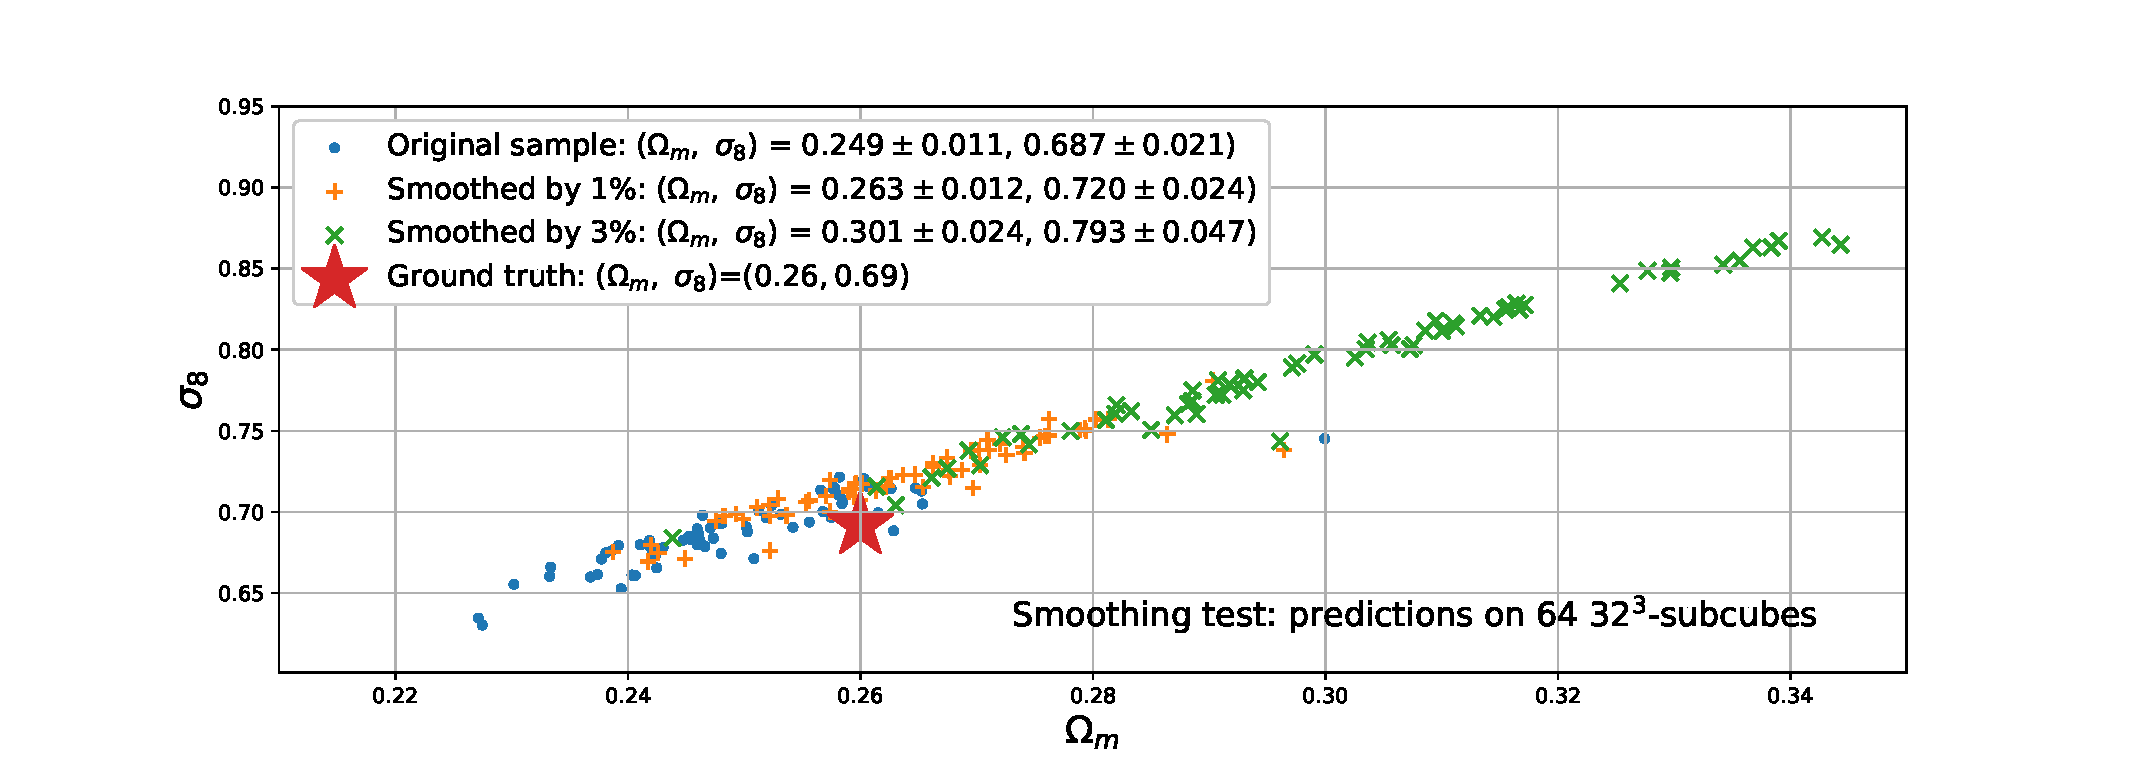
\includegraphics[width=16cm]{test_smooth.eps}
   \caption{\label{test_smooth}
   A test about error-tolerance of the CNN: sensitivity to smoothing.
   The input sample is a $128^3$-grid with cosmology $(\Omega_m, \sigma_8)=(0.26,0.69)$.
   Predictions on the 64 $32^3$-subgrids are plotted.
   The CNN can correctly predict the input cosmologies using the input sample.
   If we artificially smooth the grid by, say, 1\% and 3\% 
    (replacing the density at each voxel point by adding a fraction of the density in 6 nearby voxels to it),
    we find 2$\sigma$ error in the predictions.
   Also, the statistical error is amplified by 2 times in the 3\%-smoothing case.
   }
\end{figure*}

\begin{figure*}
   \centering
    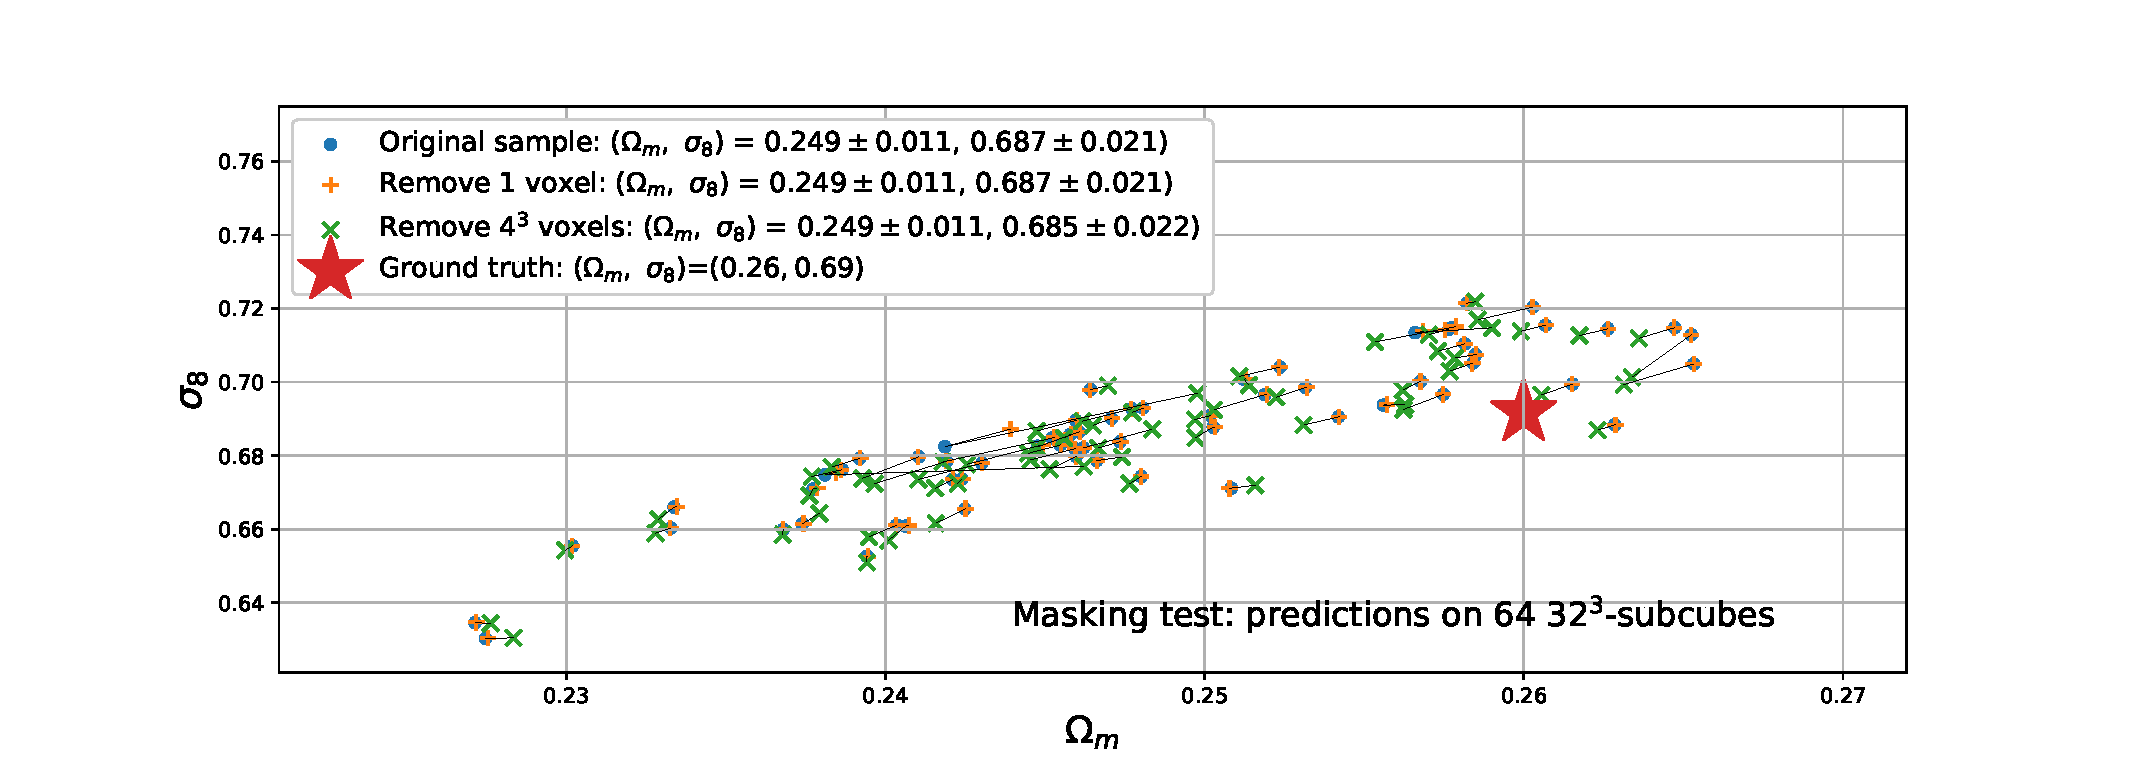
\includegraphics[width=16cm]{test_mask.eps}
   \caption{\label{test_smooth}
   A test about error-tolerance of the CNN: sensitivity to masking.
   The input sample is a $128^3$-grid with cosmology $(\Omega_m, \sigma_8)=(0.26,0.69)$.
   Predictions on the 64 $32^3$-subgrids are plotted.
   In case we mask 1 or $4^3$ voxels in each of the $32^3$-subgrid (set the values to 0), the predicted results are almost unchanged.
   This error-tolerance ability is very helpful when we apply the CNN to real observational data where there are many masked regions.
   %This is  to observation
   }
\end{figure*}

\begin{figure*}
   \centering
    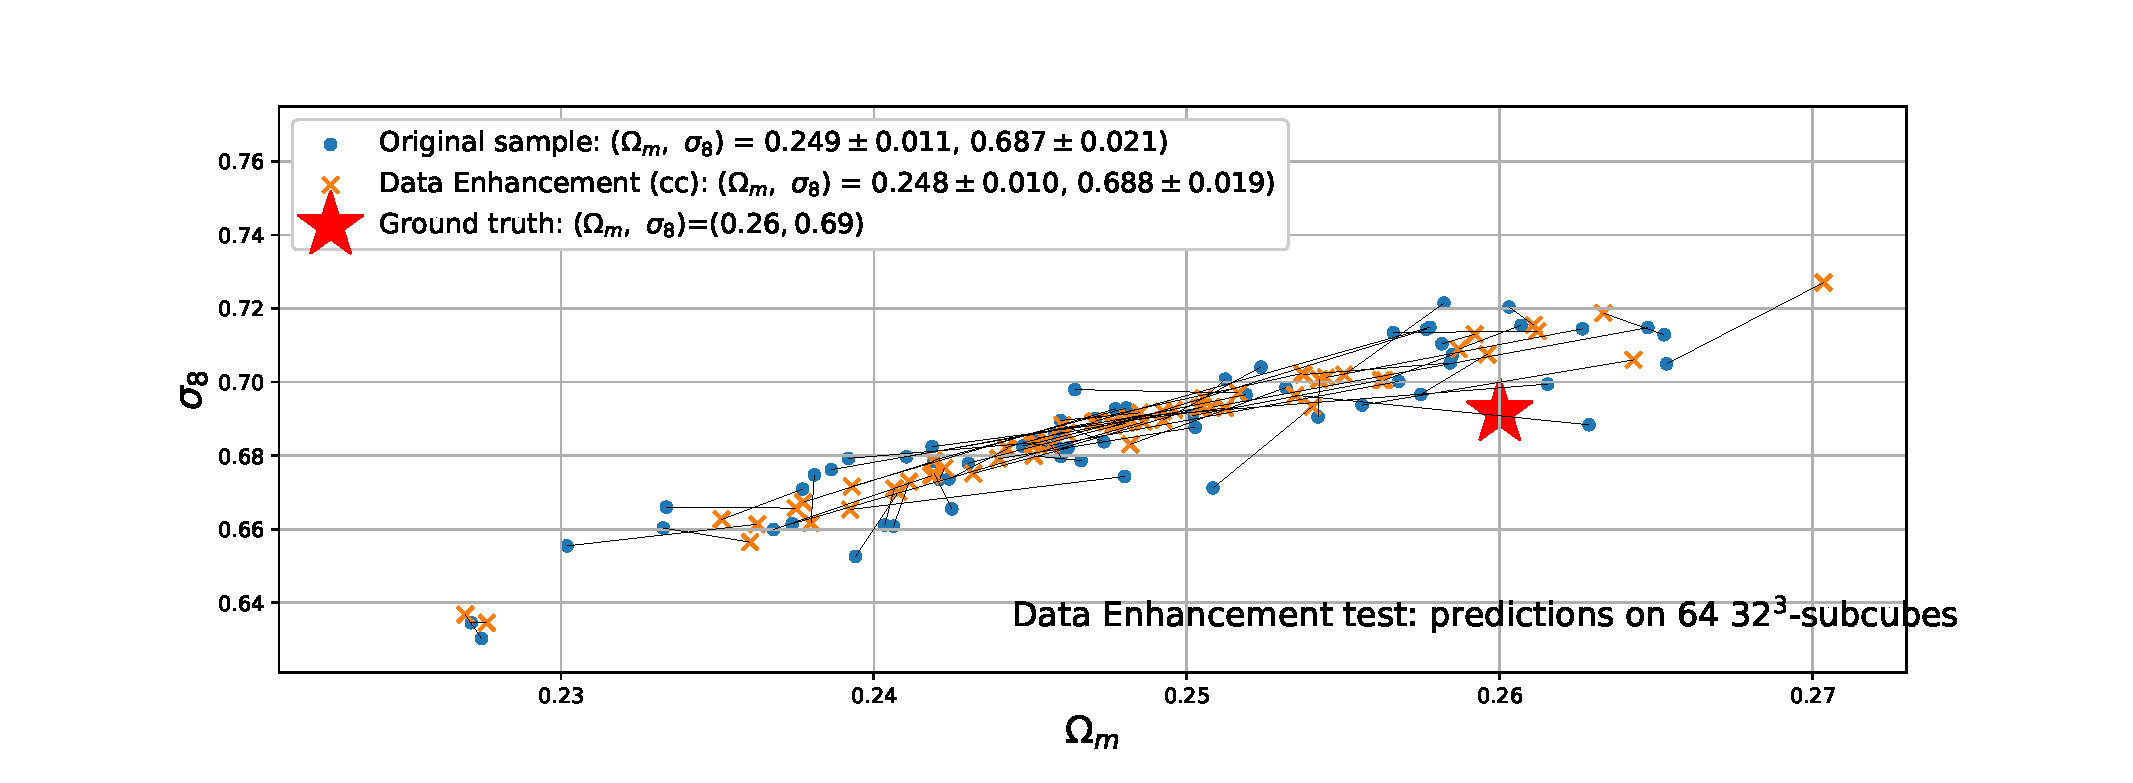
\includegraphics[width=16cm]{test_de.eps}
   \caption{\label{test_de}
   A test about using data enhancement (DE) in prediction.
   The number of test samples, after DE, is increased by as much as 48 times, yet no significant improvement in the prediction is detected.
   %The input sample is a $128^3$-grid with cosmology $(\Omega_m, \sigma_8)=(0.26,0.69)$.
   %Predictions on the 64 $32^3$-subgrids are plotted.
   %This is  to observation
   }
\end{figure*}


\begin{figure*}
   \centering
    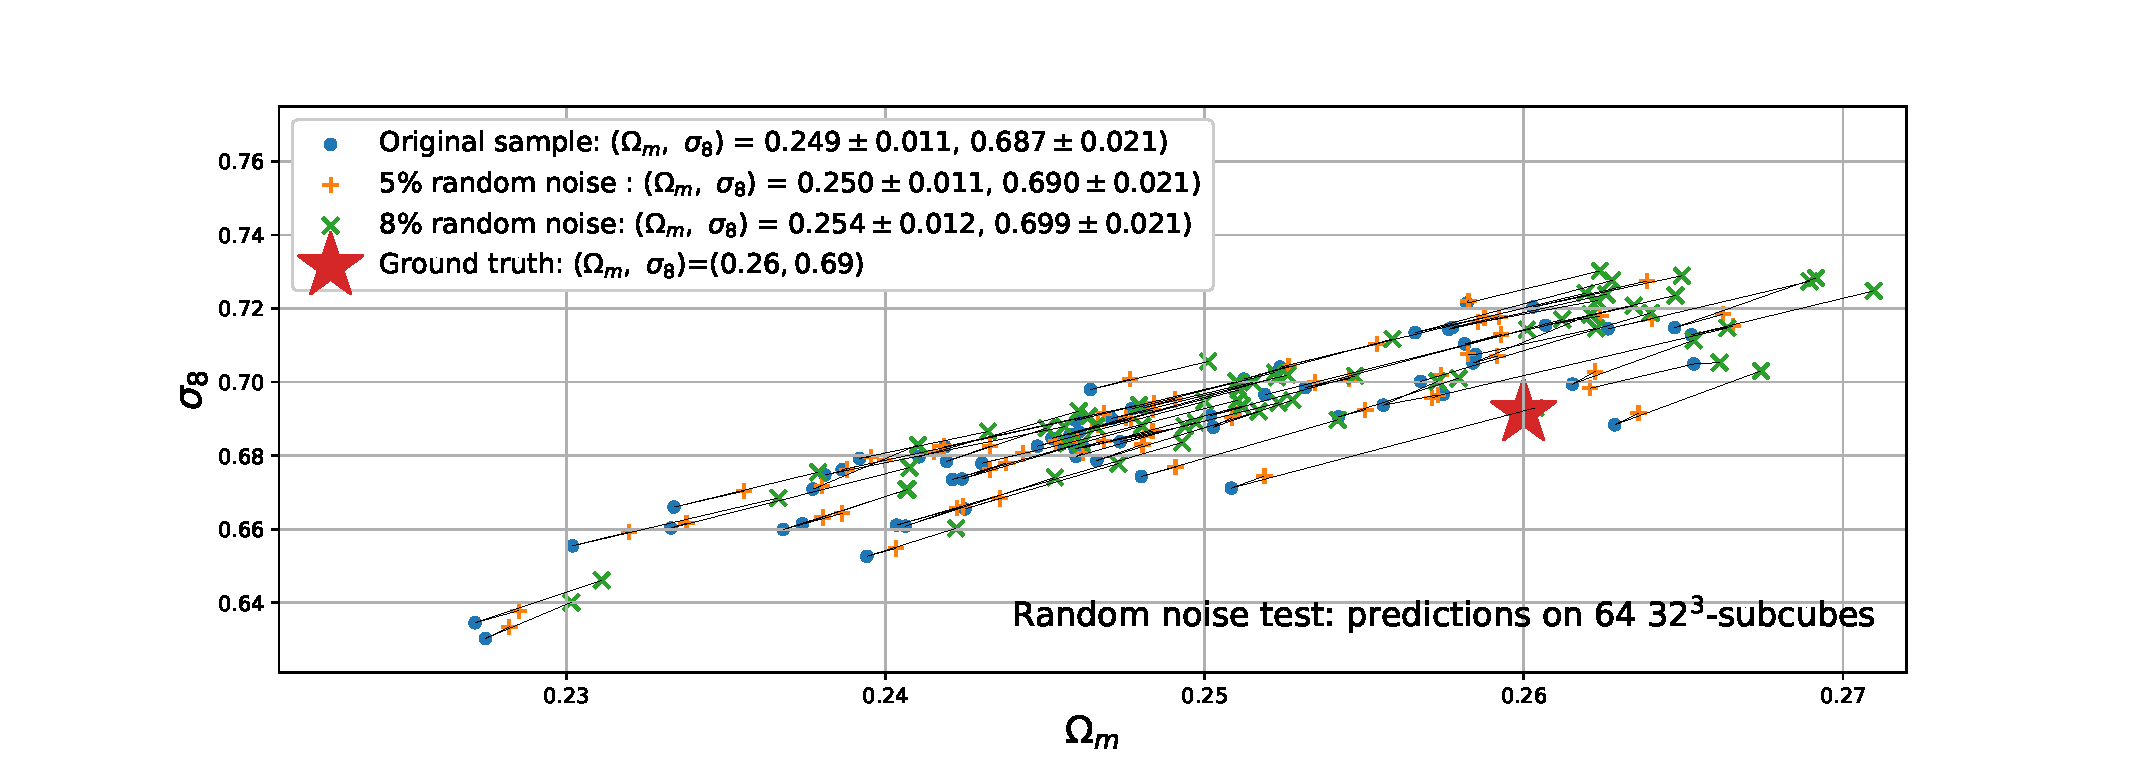
\includegraphics[width=16cm]{test_noise.eps}
   \caption{\label{test_noise}
   An error-tolerance test about noise.
   In this test, all pixels are multiplied by a Gaussian random variable with 
   mean value $\mu$=1 and $\sigma$=0.05 or 0.1.
   In both cases we do not find significant change in the prediction (well below 1$\sigma$).
   %The input sample is a $128^3$-grid with cosmology $(\Omega_m, \sigma_8)=(0.26,0.69)$.
   %Predictions on the 64 $32^3$-subgrids are plotted.
   %This is  to observation
   }
\end{figure*}

\begin{figure*}
   \centering
    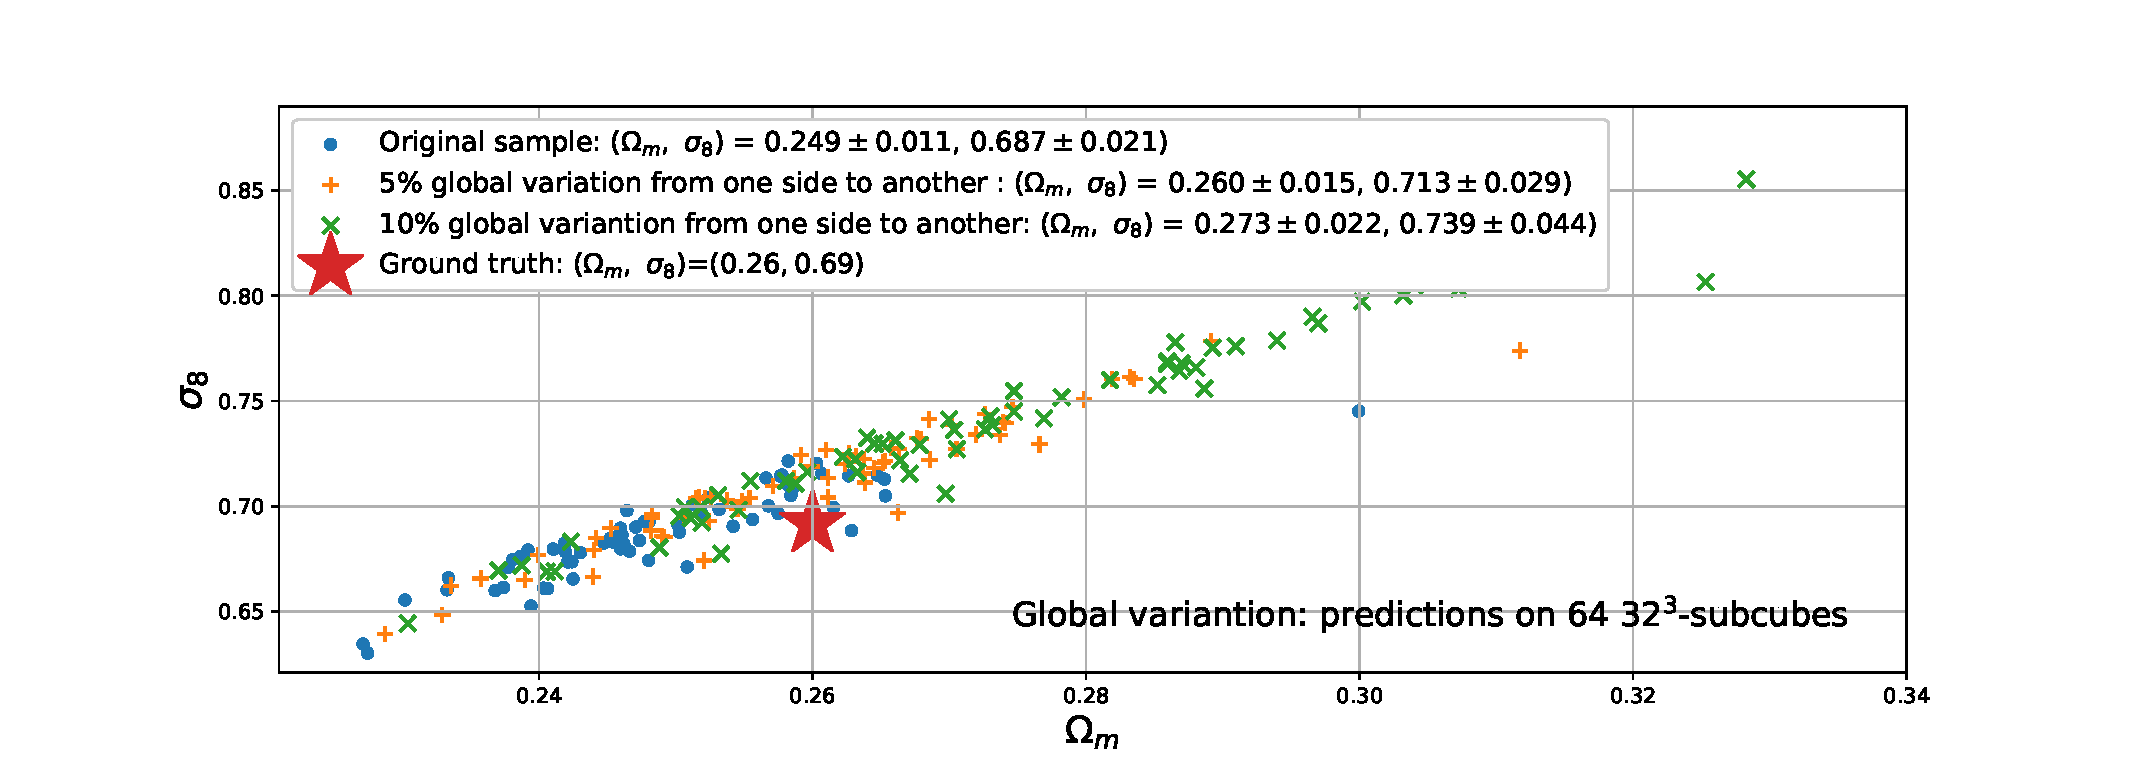
\includegraphics[width=16cm]{test_globalchange.eps}
   \caption{\label{test_globalchange}
   An error-tolerance test about global change.
   A global variation in the density field can create notable change in the predicted results.
   Cases of 5\% or 10\% change (linearly increase from 0\% at $x=0$ to 5\% or 10\% at $x=256 {h^{-1}\rm  Mpc}$) are plotted.
   In case of a 5\% change, the mean values are overestimated by (0.024, 0.052),
    and the scattering is increased by 100\%.
   In case of a 10\% change, the mean values are overestimated by (0.056, 0.11),
   while the scattering being enlarged by 4 times.
   %The input sample is a $128^3$-grid with cosmology $(\Omega_m, \sigma_8)=(0.26,0.69)$.
   %Predictions on the 64 $32^3$-subgrids are plotted.
   %This is  to observation
   }
\end{figure*}


%--------------------------------------------------------------------------------------------------------------
\section{Methodology}
\label{sec:method}

We use the following architecture...

The three convolution layers and three dense layers
have (896, 55,360, 221,312) and (1,049,600, 262,400, 514) parameters.

We varied the options...

Learning curve...

%We follow the methodology of \cite{Li2014,Li2015,Li2016},
%and perform a tomographic AP analysis on the SDSS-III BOSS DR12 galaxies.
%The results are then combined with external datasets of

%We dark energy EoS is parametrized using the non-parametric method
%{\bf CITE}.
%--------------------------------------------------------------------------------------------------------------


\section{Results}\label{sec:results}




%\begin{figure*}
%   \centering{
%   \includegraphics[width=12cm]{wz.pdf}
%   }
%   \caption{\label{fig_wz}
%   Derived redshift evolution of $w(z)$. The mean values and 68.3\%  CL regions are plotted.
%   }
%\end{figure*}



\section{Concluding Remarks}\label{sec:conclusion}




\acknowledgments


We thank Kwan-Chuen Chan, Cheng Cheng, Zhiqi Huang and  Xin Wang for many helps.
XDL acknowledges the supported from NSFC grant (No. 11803094). 





\begin{thebibliography}{}

\bibitem[Ade et al. (2015)]{Planck2015}
Ade, P.A.R., Aghanim, N., \& Arnaud, M., et al. arXiv:1502.01589

\bibitem[Aghamousa et al.(2016)]{DESI}
Aghamousa, A., 2016, arXiv:1611.00036


\bibitem[Alam et al.(2016)]{Alam2016}
Alam, S., Ata, M., \& Bailey, S., et al. 2016,
submitted to MNRAS (arXiv:1607.03155)

%\bibitem[Albrecht et al.(2006)]{DETF}
%Albrecht, A., Bernstein, G., \& Cahn, R., et al. 2006. [astro-ph/0609591].

%\bibitem[{{Alam} {et~al}\mbox{.}(2015{\natexlab{a}}){Alam}, {Albareti},
%  {Allende Prieto}, {Anders}, {Anderson}, {Anderton}, {Andrews}, {Armengaud},
%  {Aubourg}, {Bailey}, \& et~al.}]{dr12}
%{Alam} S., Albareti, F.D.,\& Allende Prieto, C., {et~al.}, 2015,  ApJS, 219, 12

\bibitem[Alcock \& Paczynski(1979)]{AP1979}
Alcock, C., \& Paczynski, B. 1979, Nature, 281, 358  
We did not discuss the systematics of the AP method in details.

%\bibitem[Anderson et al.(2012)]{2012MNRAS.427.3435A} 
%Anderson, L., Aubourg, E., Bailey, S., et al.\ 2012, MNRAS, 427, 3435

\bibitem[Anderson et al.(2013)]{Anderson2013}
Anderson, L., Aubourg, \'E., \& Bailey, S. et al. 2014, MNRAS, 441, 24  
  
%\bibitem[Bassett et al.(2002)]{Bassett2002}
%Bassett, B.A., Kunz, M., Silk, J., \& Ungarelli, C. 2002, MNRAS, 336, 1217

\bibitem[Ballinger, Peacock \& Heavens 1996]{Ballinger1996}
Ballinger, W.E., Peacock, J.A., \& Heavens, A.F. 1996, MNRAS, 282, 877  

%\bibitem[Bueno Belloso et al. (2012)]{BB2012}
%Bueno Belloso, A., Pettinari, G.W., Meures, N., \& Percival, W.J. 2012, Phys. Rev. D, 86, 023530

\bibitem[Betoule et al.(2014)]{JLA}
Betoule, M., Kessler, R., \& Guy, J., et al. 2014, A\&A, 568, 32

\bibitem[Beutler et al.(2011)]{6dFGS}
Beutler, F., Blake, C., \& Colless, M., et al. 2011, MNRAS, 416, 3017

%\bibitem[Beutler et al.(2013)]{Beutler2013}
%Beutler, F., Saito, S., \& Seo, H.-J., et al. 2013, MNRAS, 443, 1065

%\bibitem[Beutler et al.(2016)]{Beutler2016}
%Beutler, F., Seo, H.-J., \& Saito, S., et al. 2016,
%arXiv:1607.03150

\bibitem[Bond et al.(1997)]{Bond1997}
Bond, J. R., Efstathiou, G., \& Tegmark M. 1997, MNRAS, 291, L33

\bibitem[Blake et al.(2011)]{Blake2011}
Blake, C., Glazebrook, K., \& Davis, T. M., 2011, MNRAS, 418, 1725  

%\bibitem[Blake et al.(2013)]{WiggleZtopoloy}
%Blake, C., James, J.B., \& Poole, G.B. 2013, MNRAS, 437, 2488

%\bibitem[Bolton et al.(2012)]{Bolton2012}
%Bolton, A.S., Schlegel, \& D.J., Aubourg E., et al. 2012, AJ, 144, 144

%\bibitem[Boylan-Kolchin et al.(2008)]{B08}
%Boylan-Kolchin, M., Ma, C.-P., \& Quataert, E. 2008, MNRAS, 383, 93


%\bibitem[Chevallier \& Polarski(2001)]{CPL_CP}
%Chevallier, M., Polarski, D. 2001, Int. J. Mod. Phys. D, 10, 213

%\bibitem{CPL_CP}
%Chevallier, M, \& Polarski, D. 2001, Int. J. Mod. Phys. D,  10, 213


%\bibitem[Choi et al.(2010)]{choi 2010}
%Choi, Y.-Y., Park, C., Kim, J., Gott, J.R., 
%Weinberg, D.H., Vogeley, M.S., \& Kim, S.S. 2010, ApJS, 190, 181

%\bibitem[Christensen et al.(2001)]{Bayesian}
%Christensen, N., Meyer, R., Knox, L., \& Luey, B. 2001, Class. Quant. Grav., 18, 2677

\bibitem[Crittenden et al.(2012)]{Crittenden2011}
Crittenden, R.G. et al. 2012, JCAP, 02, 048

%\bibitem[Chuang et al.(2013)]{Chuang2013}
%Chuang, C.-H., Prada, F., Beutler, F., et al. 2013, arXiv:1312.4889  

%\bibitem[Chuang \& Wang(2012)]{ChuangWang2012}
%Chuang, C.-H., \& Wang, Y. 2012, MNRAS, 426, 226  


%\bibitem[Corasaniti \& Copeland(2003)]{Corasaniti2003}
%Corasaniti, P.S., Copeland, E.J. 2003, Phys. Rev. D, 67, 063521


\bibitem[Crittenden et al.(2009)]{Crittenden2009}
Crittenden, R. G., Pogosian, Li, \& Zhao, G.-B., 2009. JCAP, 0912, 025
%R. G. Crittenden, L. Pogosian and G. B. Zhao, JCAP0912 (2009) 025

\bibitem[Crittenden et al.(2012)]{Crittenden2012}
Crittenden, R. G., Zhao, G.-B., \& Pogosian, Li, et al. 2012. JCAP, 1202, 048


%eBOSS: 
%http://arxiv.org/abs/1508.04473
%\bibitem[Dawson et al.(2015)]{eBOSS}
%Dawson, K.S., Kneib, J.P., \& Percival, W.J., et al. 2015, accepted AJ

%\bibitem[Dawson et al.(2012)]{Dawson et al. 2012}
%Dawson, K.S., Schlegel, D.J., \& Ahn, C.P., et al. 2012, AJ, 145, 10


\bibitem[Delubac, T. et al.(2015)]{Deblubac2015} 
Delubac, T. et al. 2015, Astron. \& Astrophys. 574, A59
%Baryon acoustic oscillations in the Lyα forest of BOSS DR11 quasars

\bibitem[Doogesh et al.(2018)]{Doogesh2018}
Kodi Ramanah, D., Lavaux, G, Jasche, J., \& Wandelt, B.D., et al. 2019, 
A\&A, 621, A69
 

 
\bibitem[Efstathiou (2014)]{E14H0}
Efstathiou, G. 2014, MNRAS, 440, 1138

%\bibitem[Eisenstein et al.(2011)]{Eisenstein et al. 2011}
%Eisenstein, D.J.,  Weinberg, D.H., \& Agolet, E., et al. 2011, AJ, 142, 72

%\bibitem[Feldman, Kaiser \& Peacock (1994)]{1994ApJ...426...23F} 
%Feldman, H.A., Kaiser, N., \& Peacock, J.A.\ 1994, ApJ, 426, 23 

\bibitem[Feng et al.(2005)]{quintom1}
Feng, B., Wang., X. L., \& Zhang, X. M., 2005. Phys. Lett. B., 607, 35


%\bibitem[Fukugita et al. (1996)]{Fukugita1996}
%Fukugita, M., Ichikawa, T., \& Gunn, J.E., et al. 1996, AJ, 111, 1748
%Publication:	
%Astronomical Journal v.111, p.1748 

%\bibitem[Gingold \& Monaghan(1977)]{GM1977}
%Gingold, R.A., \& Monaghan, J.J. 1977, MNRAS, 181, 375  

%\bibitem[Gott et al.(2009)]{gott 2009}
%Gott, J.R., Choi, Y.-Y., Park, C., \& Kim, J. 2009, ApJ, 695, L45  

%\bibitem[Gott et al.(2008)]{gott 2008}
%Gott, J.R., Hambrick, D.C., Vogeley, M.S., Kim, J., Park, C., Choi, Y.-Y.,
%Cen, R., Ostriker, J.P., \& Nagamine, K. 2008, ApJ, 675, 16  


%\bibitem[Gunn et al. (1998)]{Gunn1998}	
%Gunn, J.E., Carr, M., \& Rockosi, C. et al. 1998, AJ, 116, 3040

%\bibitem[Gunn et al.(2006)]{Gunn et al. 2006}
%Gunn, J.E., Siegmund, W.A., \& Mannery, E.J., et al. 2006, AJ, 131, 2332

%\bibitem[Guzzo et al.(2008)]{Guzzo2008}
%Guzzo, L., Pierleoni, M., \& Meneux, B., et al. 2008, Nature, 451, 541

%\bibitem[Hamaus et al.(2016)]{2016PhRvL.117i1302H} 
%Hamaus, N., Pisani, A., Sutter, P.~M., et al.\ 2016, Physical Review Letters, 117, 091302 

%\bibitem[Hartlap et al.(2006)]{Hartlap}
%Hartlap J., Simon P. \& Schneider P. [astro-ph/0608064].

\bibitem[Heymans, C. et al.(2013)]{Heymans2013}
Heymans, C. et al. 2013, Mon. Not. R. Astron. Soc. 432,
2433–2453. 1303.1808.
%CFHTLenS tomographic weak lensing cosmological parameter constraints:
%Mitigating the impact of intrinsic galaxy alignments.

%\bibitem[Hong et al.(2016)]{hong2016}
%Hong, S.E., Park, C.,\&  Kim, J. 2016, ApJ, 823, 103

%\bibitem[Jackson (1972)]{FOG}
%Jackson, J., 1972, MNRAS, 156, 1

%\bibitem[Jennings et al.(2011)]{Jennings2011}
%Jennings, E., Baugh, C.M., \& Pascoli, S. 2011, MNRAS, 420, 1079  

%\bibitem[Joyce et al.(2015)]{2015PhR...568....1J} Joyce, A., Jain, B., Khoury, J., \& Trodden, M.\ 2015, \physrep, 568, 1 


%\bibitem[Jeong et al.(2014)]{Jeong2014}
%Jeong, D., Dai, L., Kamionkowski, M., \& Szalay, A.S. 2014, arXiv:1408.4648

%\bibitem[Jiang et al.(2008)]{jiang2008}
%Jiang, C.Y., Jing, Y. P., \& Faltenbacher, A., et al. 2008, ApJ, 675, 1095

%\bibitem[Kaiser (1987)]{Kaiser1987}
%Kaiser, N. 1987, MNRAS, 227, 1


%\bibitem[Kim \& Park(2006)]{kim and park 2006}
%Kim, J., \& Park, C. 2006, ApJ, 639, 600  

%\bibitem[Kim et al.(2009)]{2009ApJ...701.1547K} 
%Kim, J., Park, C., Gott, J.R., III, \& Dubinski, J.\ 2009, ApJ, 701, 1547 

\bibitem[Kim et al.(2015)]{HR4}
Kim, J., Park, C., L'Huillier, B., \& Hong, S. E. 2015, JKAS, 48, 213

%\bibitem[Kim et al.(2011)]{horizonrun}
%Kim, J., Park, C., Rossi, G., Lee, S.M., \& Gott, J.R. 2011, JKAS, 44, 217  

\bibitem[Kitaura et al.(2015)]{MDPATCHY}
Kitaura, F.S., Rodriguez-Torres, S., Chuang, C.-H., et al. arXiv:1509.06400

%\bibitem[Klypin et al.(2016)]{K2014}
%Klypin, A., Yepes, G., Gottlober, S., Prada, F., \& Hess, S. 2016,
%MNRAS, 457, 4340%

%\bibitem[Komatsu et al.(2011)]{komatsu2011}
%Komatsu, E., Smith, K. M., \& Dunkley, J., et al. 2011, ApJS, 192, 18  

%\bibitem[Lacey \& Cole(1993)]{LC93}
%Lacey, C., \& Cole, S. 1993, MNRAS, 262, 627


%\bibitem[Landy \& Szalay(1993)]{1993ApJ...412...64L} 
%Landy, S.D., \& Szalay, A.S.\ 1993, ApJ, 412, 64 

%EUCLID:
%http://arxiv.org/abs/1110.3193
\bibitem[Laureijs et al.(2011)]{EUCLID}
Laureijs, R., Amiaux, J., \& Arduini, S., et al. 2011, arXiv:1110.3193

%\bibitem[Lavaux \& Wandelt(2012)]{LavausWandelt1995}
%Lavaux, G., \& Wandelt, B.D. 2012, ApJ, 754, 109  

\bibitem[Lavaux \& Wandelt(2012)]{LavausWandelt2012}
Lavaux, G., \& Wandelt, B.D. 2012, ApJ, 754, 109

%\bibitem[Levi et al.(2013)]{2013arXiv1308.0847L} 
%Levi, M., Bebek, C., Beers, T., et al.\ 2013, arXiv:1308.0847 

%\bibitem[Lewis \& Bridle (2002)]{LB2002}
%Lewis, A., \& Bridle, S. 2002, Phys. Rev. D, 66, 103511

%\bibitem[L'Huillier et al.(2014)]{2014NewA...30...79L} 
%L'Huillier, B., Park, C., \& Kim, J.\ 2014, New Astronomy, 30, 79 

\bibitem[Li et al.(2011)]{Li2011}
Li, M., Li, X.-D., Wang, S., \& Wang, Y. 2011, Commun. Theor. Phys., 56, 525

\bibitem[Li et al.(2014)]{Li2014}
Li, X.-D., Park, C., Forero-Romero, J., \& Kim, J. 2014, ApJ, 796, 137

\bibitem[Li et al.(2015)]{Li2015}
Li, X.-D., Park, C., Sabiu, C.G., \& Kim, J. 2015, MNRAS, 450, 807 

\bibitem[Li et al.(2016)]{Li2016}%
Li, X.-D., Park, C., \& Sabiu, C.G., et al. 2016, ApJ, 832, 103

\bibitem[Li et al.(2018)]{Li2018}%
Li, X.-D., Sabiu, C.G., \& Park, C., et al. 2018, ApJ, 856, 88

\bibitem[Li et al.(2019)]{Li2019}%
Li, X.-D., Miao, H, \& Wang, X., et al. 2019, submitted to ApJ, arXiv:1903.04757


%\bibitem[Linder(2003)]{CPL_L}
%Linder, E.V. 2003, Phys. Rev. Lett., 90, 091301

%\bibitem[Linder et al.(2014)]{Linder2013}
%Linder, E.V., Minji, O., Okumura, T., Sabiu, C.G., \& Song, Y.-S. 2014, Phys. Rev. D, 89, 063525  

%\bibitem[L{\'o}pez-Corredoira(2014)]{2014ApJ...781...96L} 
%L{\'o}pez-Corredoira, M.\ 2014, ApJ, 781, 96 

\bibitem[Mao et al. (2016)]{Qingqing2016}
Mao, Q., Berlind, A.A., Scherrer, R.J., et al. 2016, submitted to ApJ

%\bibitem[Marinoni \& Buzzi(2010)]{Marinoni2010}
%Marinoni, C., \& Buzzi, A. 2010, Nature, 468, 539  


\bibitem[Marco Raveri (2019)]{Marco2019}
Marco R., 2019, arXiv:1902.01366 

\bibitem[Marshall et al.(2017)]{LSST}
Marshall, Phil, Anguita, Timo, \& Bianco, F. B., et al. 2017, arXiv:1708.04058

\bibitem[Matsubara \& Suto(1996)]{Matsubara1996}
Matsubara T., \& Suto, Y. 1996, ApJ, 470, L1  

%\bibitem[McCavana et al.(2012)]{M12}
%McCavana, T., Micic, M., Lewis, G. F., et al. 2012, MNRAS, 424, 361


%\bibitem[Morandi \& Sun (2016)]{MS2016}
%Morandi, A., \& Sun, M. arXiv:1601.03741

\bibitem[Moresco, M. et al.(2016)]{Moresco2016}
Moresco, M. et al. 2016, J. Cosmol. Astropart. Phys. 5, 014. 1601.
01701.
%A 6\% measurement of the Hubble parameter at z ̃0.45: direct evidence of the epoch of cosmic re-acceleration. 

\bibitem[Outram et al.(2004)]{Outram2004}
Outram, P.J., Shanks, T., Boyle, B.J., Croom, S.M., Hoyle, F., Loaring, N.S., 
Miller, L., \& Smith, R.J. 2004, MNRAS, 348, 745  

%\bibitem[Parejko et al.(2013)]{Parejko2013}
%Parejko, J. K., Sunayama, T., Padmanabhan, N., et al. 2013, MNRAS, 429, 98  

%\bibitem[Parejko et al.(2013)]{Parejko2013}
%Parejko J.K., et al., 2013, MNRAS, 429, 98

%\bibitem[Parihar et al. (2014)]{CMASSLSS2014}
%Parihar, P., Vogeley, M.S., \& Gott, J.R., et al. 2014, ApJ, 796, 86

%\bibitem[Park et al.(2005)]{park 2005}
%Park, C., Kim, J., \& Gott, J.R. 2005, ApJ, 633, 1  

\bibitem[Park \& Kim(2010)]{topology}
Park, C., \& Kim, Y.-R. 2010, ApJL, 715, L185  

%\bibitem[Park et al.(2018)]{park18}
%Park, H., et al., 2018, {\em in preparation}

\bibitem[Parkinson, D. et al.(2012)]{Parkinson2012}
Parkinson, D. et al. 2012, Phys. Rev. D 86, 103518. 1210.2130.
%The WiggleZ Dark Energy Survey: Final data release and cosmological results
%\bibitem[Park et al. (2012)]{Park2012}
%Park, C., Choi, Y.-Y., Kim, J., Gott, J.R., Kim, S.S., \&
%Kim, K.-S. 2012, ApJ, 759, 7

%\bibitem[Park et al. (2015)]{Park2015}
%Park, C., Song, H., Einasto, M., Lietzen, H., \&
%Heinamaki, P. 2015, JKAS, 48, 75

%\bibitem[Peebles \& Ratra(2003)]{PR2003}
%Peebles, P.J.E., \& Ratra, B. 2003, Reviews of Modern Physics, 75, 559

%\bibitem[Percival et al.(2014)]{Percival2014}
%Percival, W.J., Ross, A.J., \& S\'{a}nchez, A.G., et al. 2014, MNRAS, 439, 2531

\bibitem[Perlmutter et al.(1999)]{Perl1999}
Perlmutter, S., Aldering, G., \& Goldhaber, G., et al. 1999, ApJ, 517, 565  

%\bibitem[Press \& Shechter(1974)]{PS1974}
%Press, W.H., \& Schechter, P.L. 1974, ApJ, 187, 425



%\bibitem[Reid et al.(2012)]{Reid2012}
%Reid, B., Samushia, L., \& White, M., et al. 2012, MNRAS, 426, 2719  

%\bibitem[Reid et al.(2016)]{Reidetal:2016}
%Reid, B., Ho, S., \& Padmanabhan, N., et al.  2016, MNRAS, 455, 1553

\bibitem[Ravanbakhsh et al.(2017)]{Ravanbakhsh2017}
Ravanbakhsh, S., Oliva, J., Fromenteau, S., et al. 2017, arXiv:1711.02033

\bibitem[Riess et al.(1998)]{Riess1998}
Riess, A.G., Filippenko, A.V., \& Challis, P., et al. 1998, AJ, 116, 1009  

\bibitem[Riess et al.(2011)]{Riess2011}
Riess, A.G., Macri, L., \& Casertano, S., et al. 2011, ApJ, 730, 119
%A 3\% Solution: Determination of the Hubble Constant with the Hubble Space Telescope and Wide Field Camera

%\bibitem[Ross et al.(2012)]{2012MNRAS.424..564R} 
%Ross, A.J., Percival, W.J., \& S{\'a}nchez, A.G. et al.\ 2012, MNRAS, 424, 564 

\bibitem[Ross et al.(2015)]{MGS}
Ross, A.J., Samushia, L., \& Howlett, C., et al. 2015, MNRAS, 449, 835

\bibitem[Ryden(1995)]{Ryden1995}
Ryden, B.S. 1995, ApJ, 452, 25  

%%\bibitem[Samushia et al.(2014)]{Samushia2014}
%Samushia, L., Reid, B. A., White, M., et al. 2014, MNRAS, 439, 3504  

%\bibitem[Sanchez et al.(2013)]{Sanchez2013}
%Sanchez, A. G., Kazin, E. A., Beutler, F., et al. 2013, MNRAS, 433, 1202  

%\bibitem[Sutter et al.(2014)]{Sutter2014}
%Sutter, P.M., Pisani, A., Wandelt, B.D., \& Weinberg, D.H. 2014, MNRAS, 443, 2983


%\bibitem[Sanchez et al.(2016)]{Sanchez2016}
%Sanchez, A. G., Scoccimarro, R., \& Crocce, M., et al.
%arXiv:1607.03147

%\bibitem[Schlafly et al.(2010)]{Schlafly2010}
%Schlafly E.F., Finkbeiner D.P., Schlegel D.J., et al. 2010, ApJ, 725, 1175

%\bibitem[Schlafly \& Finkbeiner(2011)]{SF2011}
%Schlafly E.F., \& Finkbeiner D.P. 2011, ApJ, 737, 103


%DESI:
%http://arxiv.org/abs/1106.1706
%\bibitem[Schlegel et al.(2011)]{DESI}
%Schlegel, D., Abdalla, F., \& Abraham, T., et al. 2011, arXiv:1106.1706

%\bibitem[Smee et al.(2013)]{Smee2013}
%Smee, S.A., Gunn, J.E., \& Uomoto, A., et al. 2013, AJ, 146, 32

%\bibitem[Song et al.(2014)]{2014arXiv1407.2257S} 
%Song, Y.S., Sabiu, C.G., 
%Okumura, T., Oh, M., \& Linder, E.V.\ 2014, JCAP, 12, 005 

%\bibitem[Speare et al. (2015)]{Speare2015}
%Speare, R., Gott, J.R., Kim, J., \& Park, C.
%2015, ApJ, 799, 176

%\bibitem[Tojeiro \& Percival(2011)]{Tojeiro2011}
%Tojeiro R., \& Percivial W.J. 2011, MNRAS, 417, 1114  

%\bibitem[Tojeiro et al.(2012)]{Tojeiro2012}
%Tojeiro, R., Percival, W. J., Wake, D. A., et al. 2012, MNRAS, 424, 136 

%\bibitem[Viana \& Liddle(1996)]{VL1996}
%Viana, P.T.P., \& Liddle, A.R. 1996, MNRAS, 281, 323

%\bibitem[Villalobos et al.(2013)]{V13}
%Villalobos, \'{A}., ÃÅ%De Lucia, G., Weinmann, S.M., Borgani, S., \& Murante, G. 2013, MNRAS, 433, L49


\bibitem[Weinberg (1989)]{SW1989}
Weinberg, S. 1989, Reviews of Modern Physics, 61, 1

\bibitem[Weinberg et al. (2013)]{DHW2013}
Weinberg, D.H, Mortonson, M.J., Eisenstein, D.J., et al. 2013, Physics Reports, 530, 87

%\bibitem[White (2011)]{White2011}
%White M., et al. 2011, ApJ, 728, 126
\bibitem[Wang et al.(2018)]{Wang:2018fng}
Wang, Y., Pogosian, L., Zhao, G.-B., \& Zucca, A. 2018. accepted by ApJL
%@article{Wang:2018fng,
%      author         = "Wang, Yuting and Pogosian, Levon and Zhao, Gong-Bo and
%                        Zucca, Alex",
%      title          = "{Evolution of dark energy reconstructed from the latest
%                        observations}",
%      doi            = "10.3847/2041-8213/aaf238",
%      year           = "2018",
%      eprint         = "1807.03772",
%      archivePrefix  = "arXiv",
%      primaryClass   = "astro-ph.CO",
%      SLACcitation   = "%%CITATION = ARXIV:1807.03772;%%"
%}

\bibitem[Yoo \& Watanabe(2012)]{2012IJMPD..2130002Y}%
Yoo, J., \& Watanabe, Y.\ 2012, International Journal of Modern Physics D, 21, 1230002 



\bibitem[Zhang et al.(2018)]{zhangxue2018} 
Zhang, X., Huang, Q.-G., \& Li, X.-D.\ 2018. Mon. Not. R. Astron. Soc., 483, 1655

%\bibitem[York et al.(2000)]{York et al. 2000}
%York, D.G., Adelman, J., \& Anderson, J.E., et al. 2000, AJ, 120, 1579

%\bibitem[Zehavi et al.(2011)]{zehavi2011}
%Zehavi, I., Zheng, Z., \& Weinberg, D.H., et al. 2011, ApJ, 736, 59

\bibitem[Zhao et al.(2012)]{zhao2012}
Zhao, G.-B., Crittenden, R.-G., Pogosian, L., \& Zhang, X, 2012. Phys. Rev. Lett., 109, 171301
%@article{Zhao:2012aw,
%      author         = "Zhao, Gong-Bo and Crittenden, Robert G. and Pogosian,
%                        Levon and Zhang, Xinmin",
%      title          = "{Examining the evidence for dynamical dark energy}",
%      journal        = "Phys. Rev. Lett.",
%      volume         = "109",
%      year           = "2012",
%      pages          = "171301",
%      doi            = "10.1103/PhysRevLett.109.171301",
%      eprint         = "1207.3804",
%      archivePrefix  = "arXiv",
%      primaryClass   = "astro-ph.CO",
%      SLACcitation   = "%%CITATION = ARXIV:1207.3804;%%"
%}

\bibitem[Zhao et al.(2017)]{Zhao:2017cud}
Zhao, G.-B., Raveri, M., \& Pogosian, L., et al. 2017, Nat. Astron., 1, 627
%Gong-Bo Zhao, Marco Raveri, Levon Pogosian, 

\bibitem[Zhao, G.-B. et al.(2017)]{ZhaoGB:2017}
Zhao, G.-B. et al. 2017, Mon. Not. R. Astron. Soc. 466, 762
%The clustering of galaxies in the completed SDSS-III Baryon Oscillation Spectroscopic Survey: tomographic BAO analysis of DR12 combined sample in Fourier space.

\bibitem[\protect\citeauthoryear{Zhao, et al.}{2019}]{2019MNRAS.482.3497Z} 
Zhao, G.-B. et al. 2019, MNRAS, 482, 3497

%@article{Zhao:2017cud,
%      author         = "Zhao, Gong-Bo and others",
%      title          = "{Dynamical dark energy in light of the latest
%                        observations}",
%      journal        = "Nat. Astron.",
%      volume         = "1",
%      year           = "2017",
%      number         = "9",
%      pages          = "627-632",
%      doi            = "10.1038/s41550-017-0216-z",
%      eprint         = "1701.08165",
%      archivePrefix  = "arXiv",
%      primaryClass   = "astro-ph.CO",
%      SLACcitation   = "%%CITATION = ARXIV:1701.08165;%%"
%}


%###########################




%3. Delubac, T. et al. Ba1ryon acoustic oscillations in the Lyα forest of BOSS DR11 quasars.
%Astron. \& Astrophys. 574, A59 (2015).

%23. Zhao, G.-B. et al. The clustering of galaxies in the completed SDSS-III Baryon Oscillation
%Spectroscopic Survey: tomographic BAO analysis of DR12 combined sample in Fourier space.
%Mon. Not. R. Astron. Soc. 466, 762–779 (2017).

%42. Parkinson, D. et al. The WiggleZ Dark Energy Survey: Final data release and cosmological
%results. Phys. Rev. D 86, 103518 (2012). 1210.2130.

%43. Heymans, C. et al. CFHTLenS tomographic weak lensing cosmological parameter constraints:
%Mitigating the impact of intrinsic galaxy alignments.
%Mon. Not. R. Astron. Soc. 432,
%2433–2453 (2013). 1303.1808.

%44. Moresco, M. et al. A 6\% measurement of the Hubble parameter at z ̃0.45: direct evidence
%of the epoch of cosmic re-acceleration. J. Cosmol. Astropart. Phys. 5, 014 (2016). 1601.
%01701.


\end{thebibliography}


\end{document}
